\chapter{Numerical experiments}\label{sec:numerical_experiments}
%------------------------------------------------------------------------------
\section{0-D, sources and sinks}\label{sec:0d_numerical_experiments}
In this section the numerical results are given for the
0-dimensional air pollution example as described in \autoref{sec:air_pollution}
and for the Brusselator, as described in \autoref{sec:brusselator}.
%------------------------------------------------------------------------------
\subsection{Air pollution}
%--------------------------------------------------------------------------------
Some numerical results of the air pollution example (\autoref{sec:air_pollution}) is:
\begin{figure}[H]
    \begin{subfigure}{0.5\textwidth}
        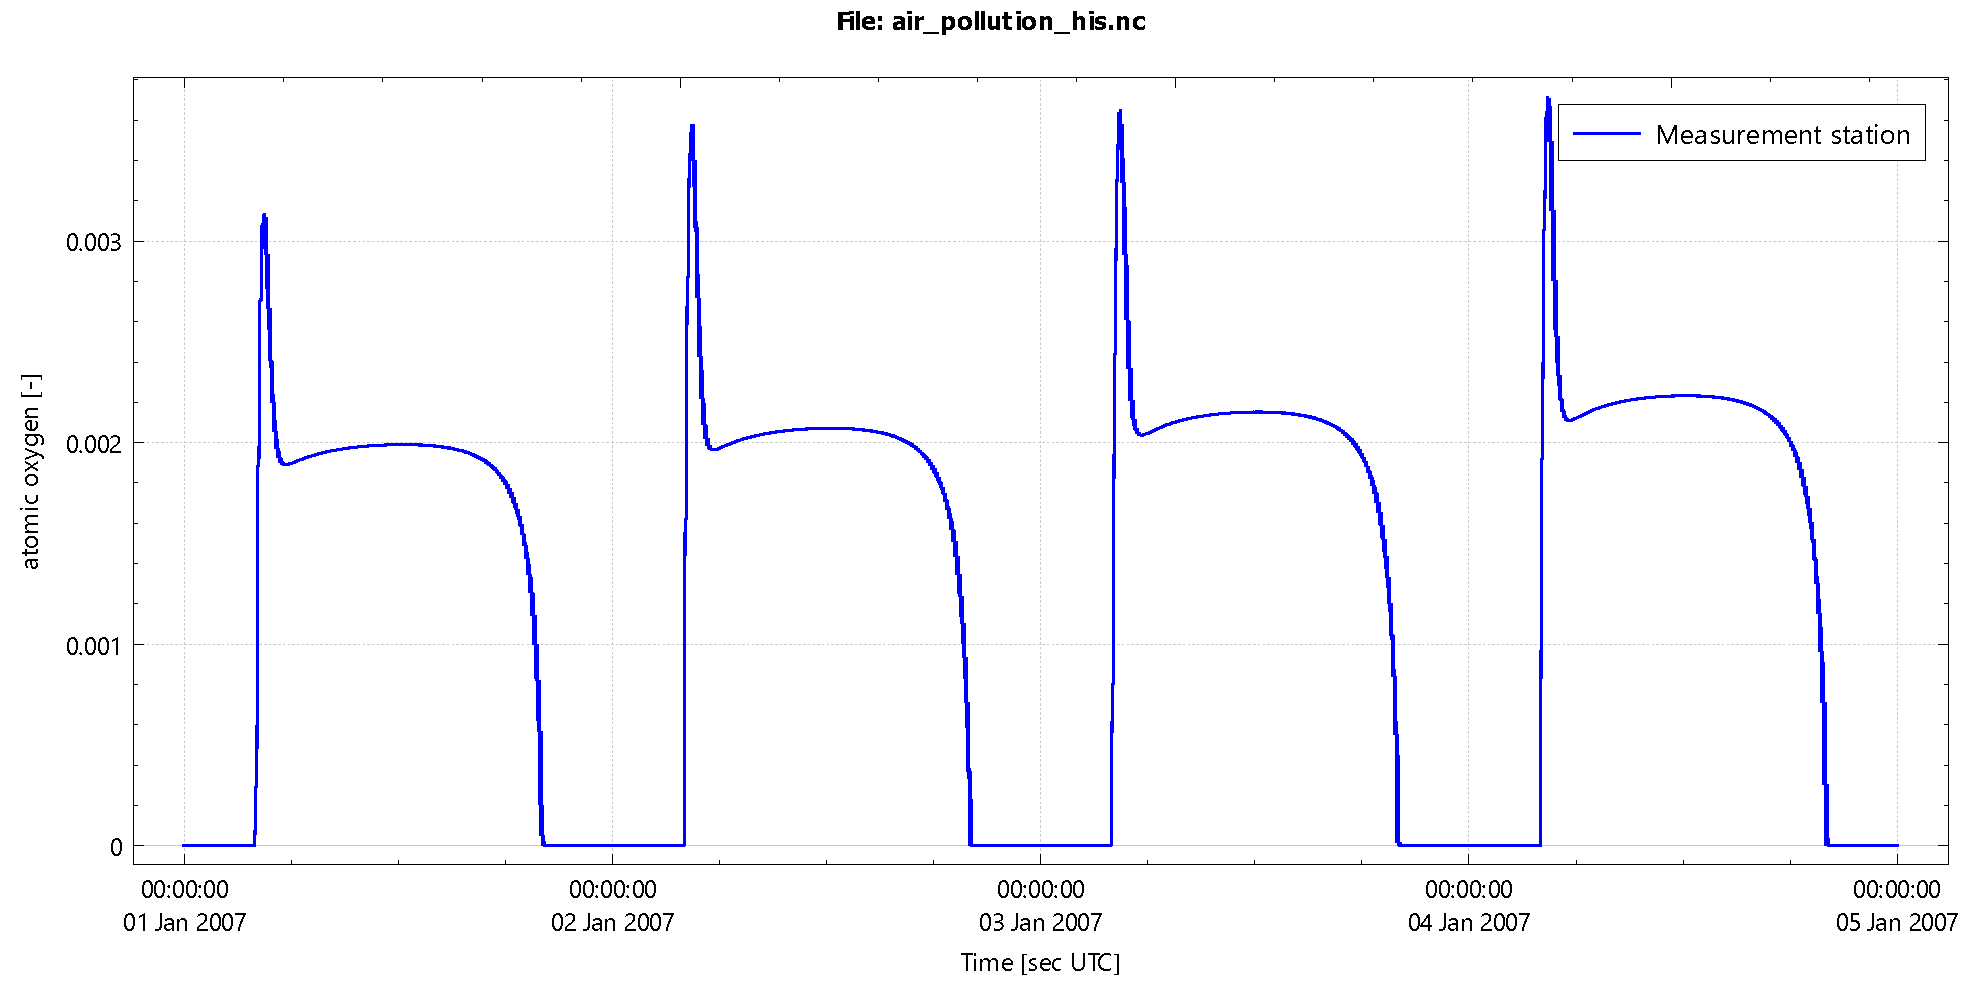
\includegraphics[width=\textwidth]{figures/atomic_oxygen_dt0d5.pdf}
        \caption{Concentration of Atomic Oxygen.}
    \end{subfigure}
    \begin{subfigure}{0.5\textwidth}
        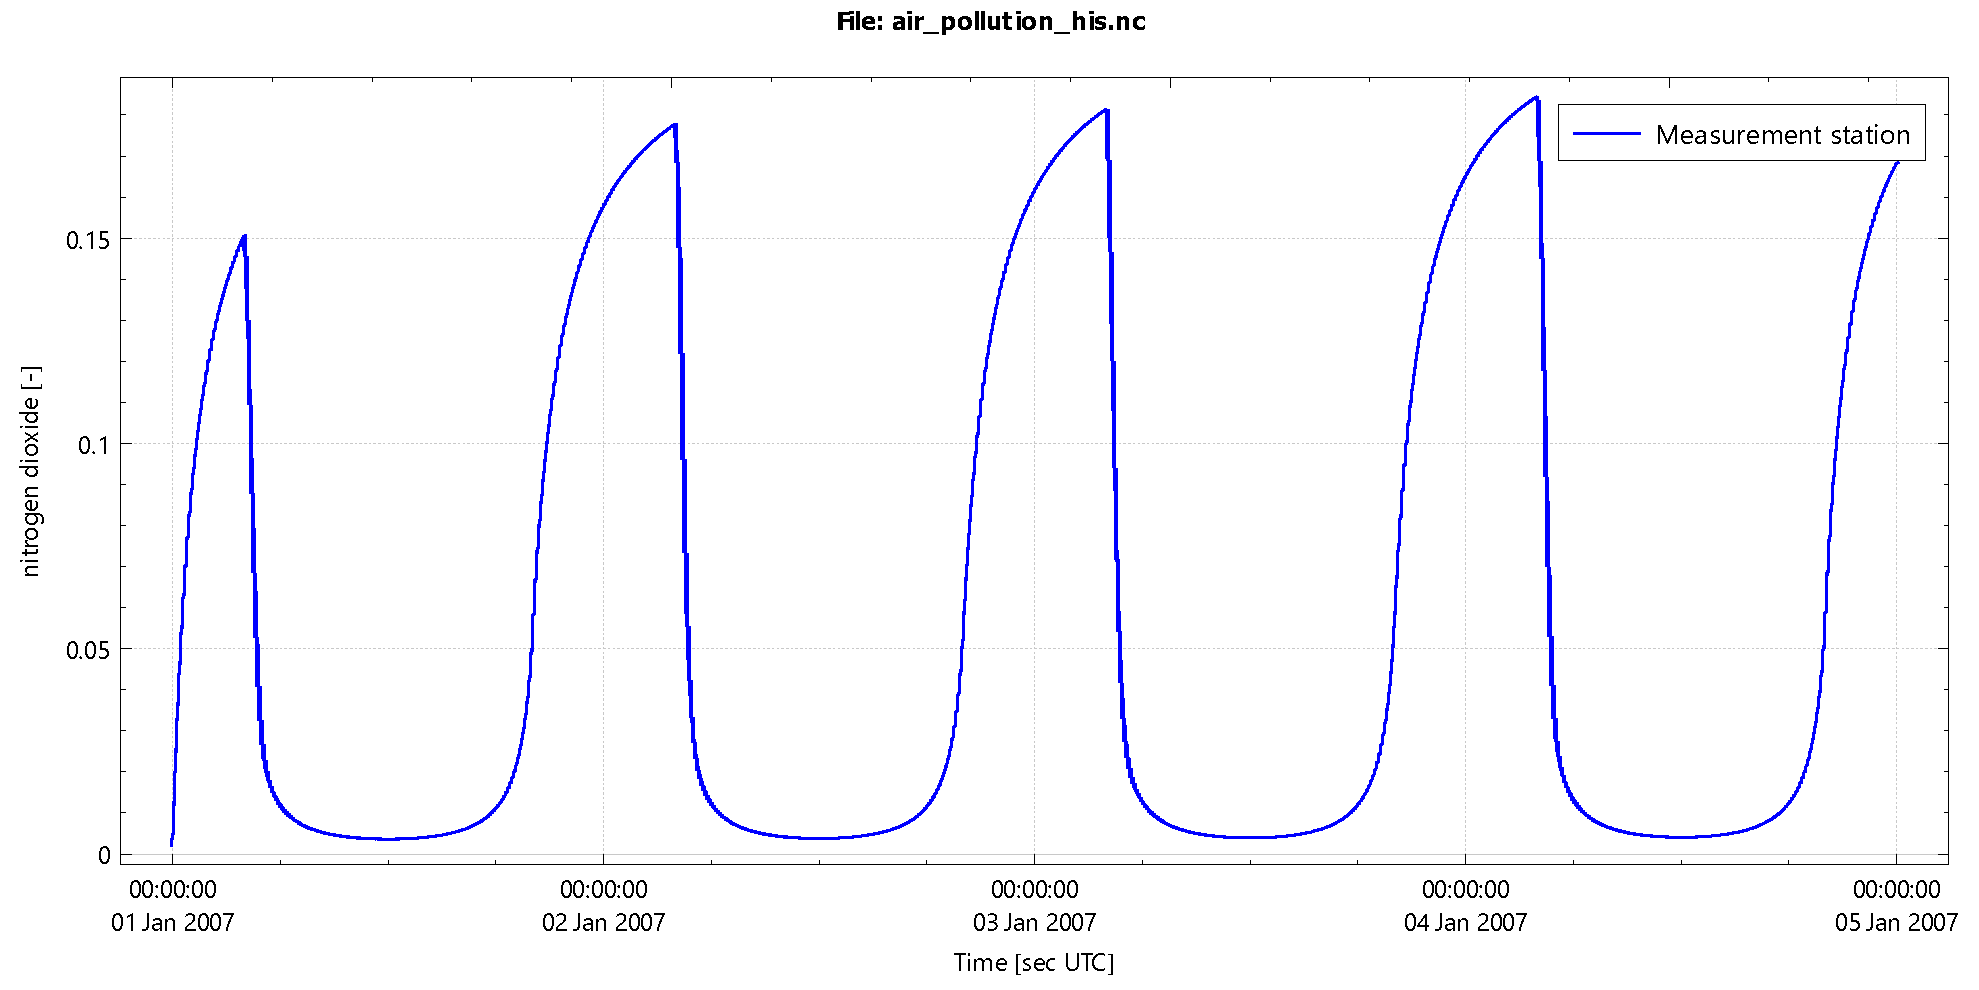
\includegraphics[width=\textwidth]{figures/nitrogen_dioxide_dt0d5.pdf}
        \caption{Concentration of Nitrogen Dioxide.}
    \end{subfigure}
    \begin{subfigure}{0.5\textwidth}
        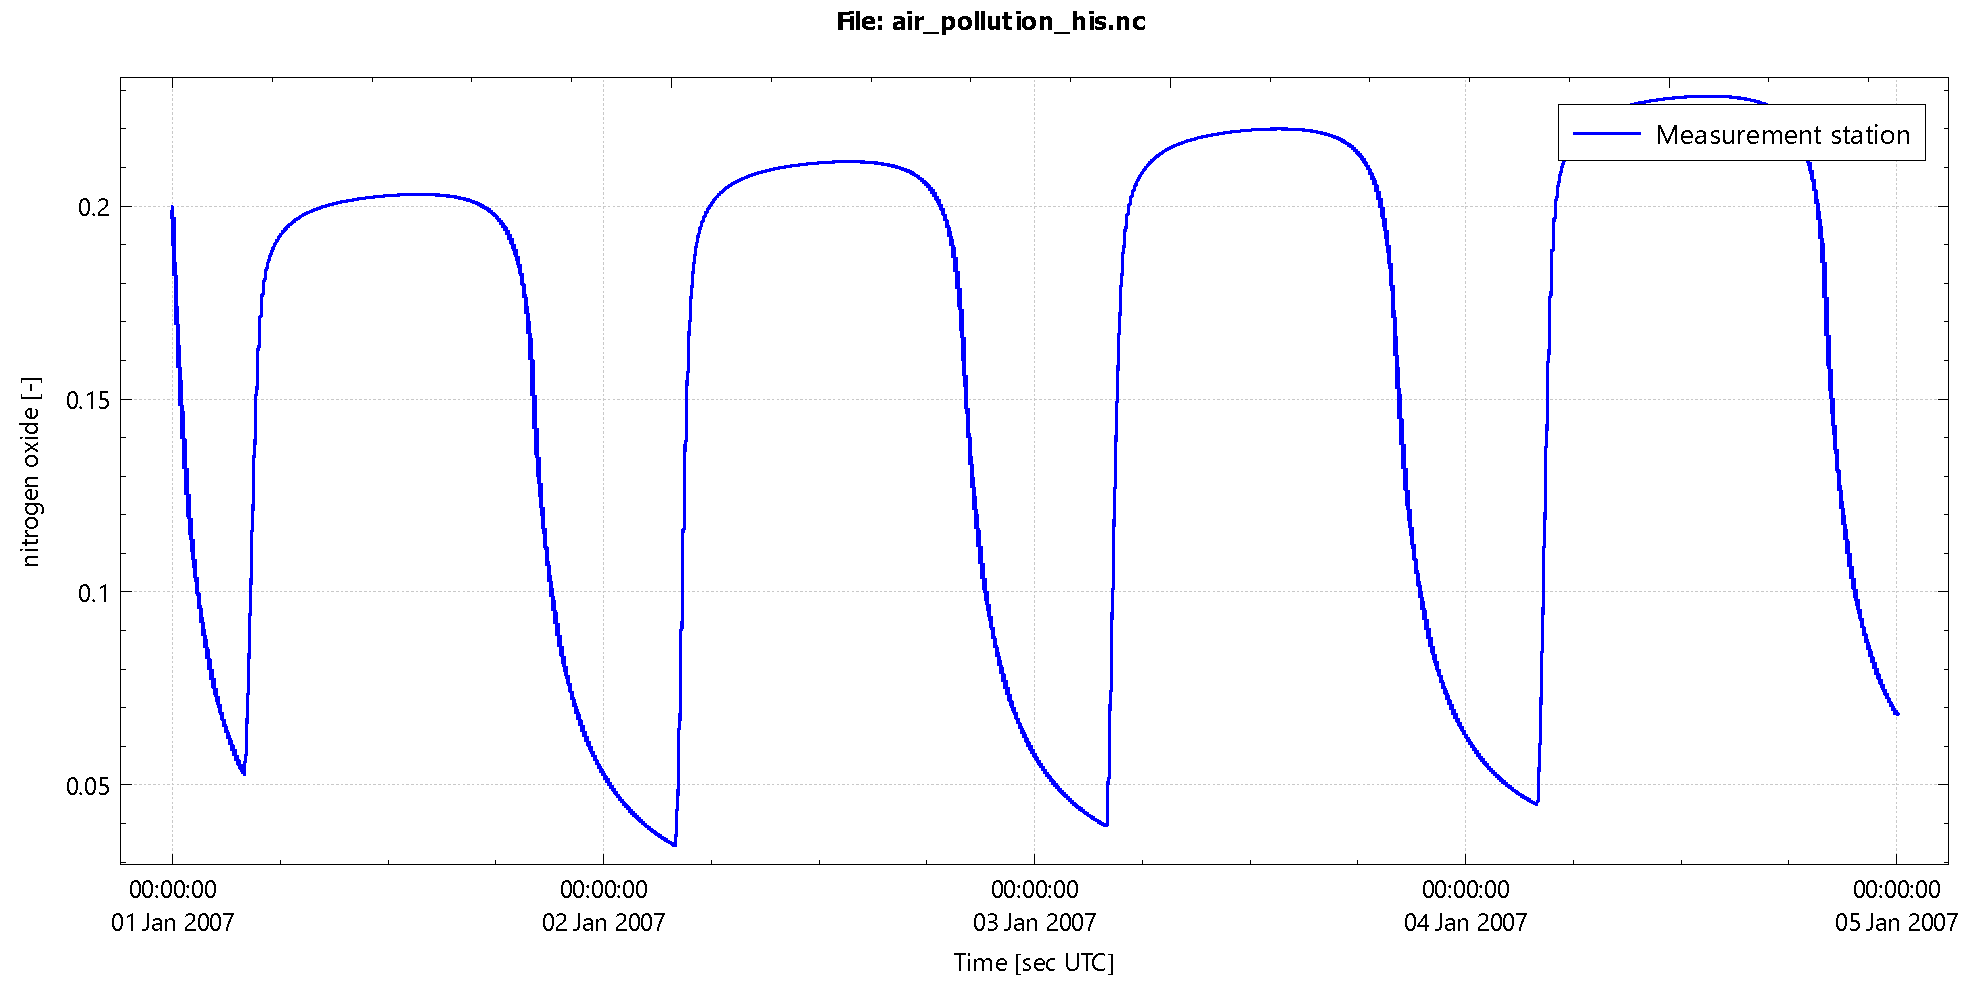
\includegraphics[width=\textwidth]{figures/nitrogen_oxide_dt0d5.pdf}
        \caption{Concentration of Nitrogen Oxide.}
    \end{subfigure}
    \begin{subfigure}{0.5\textwidth}
        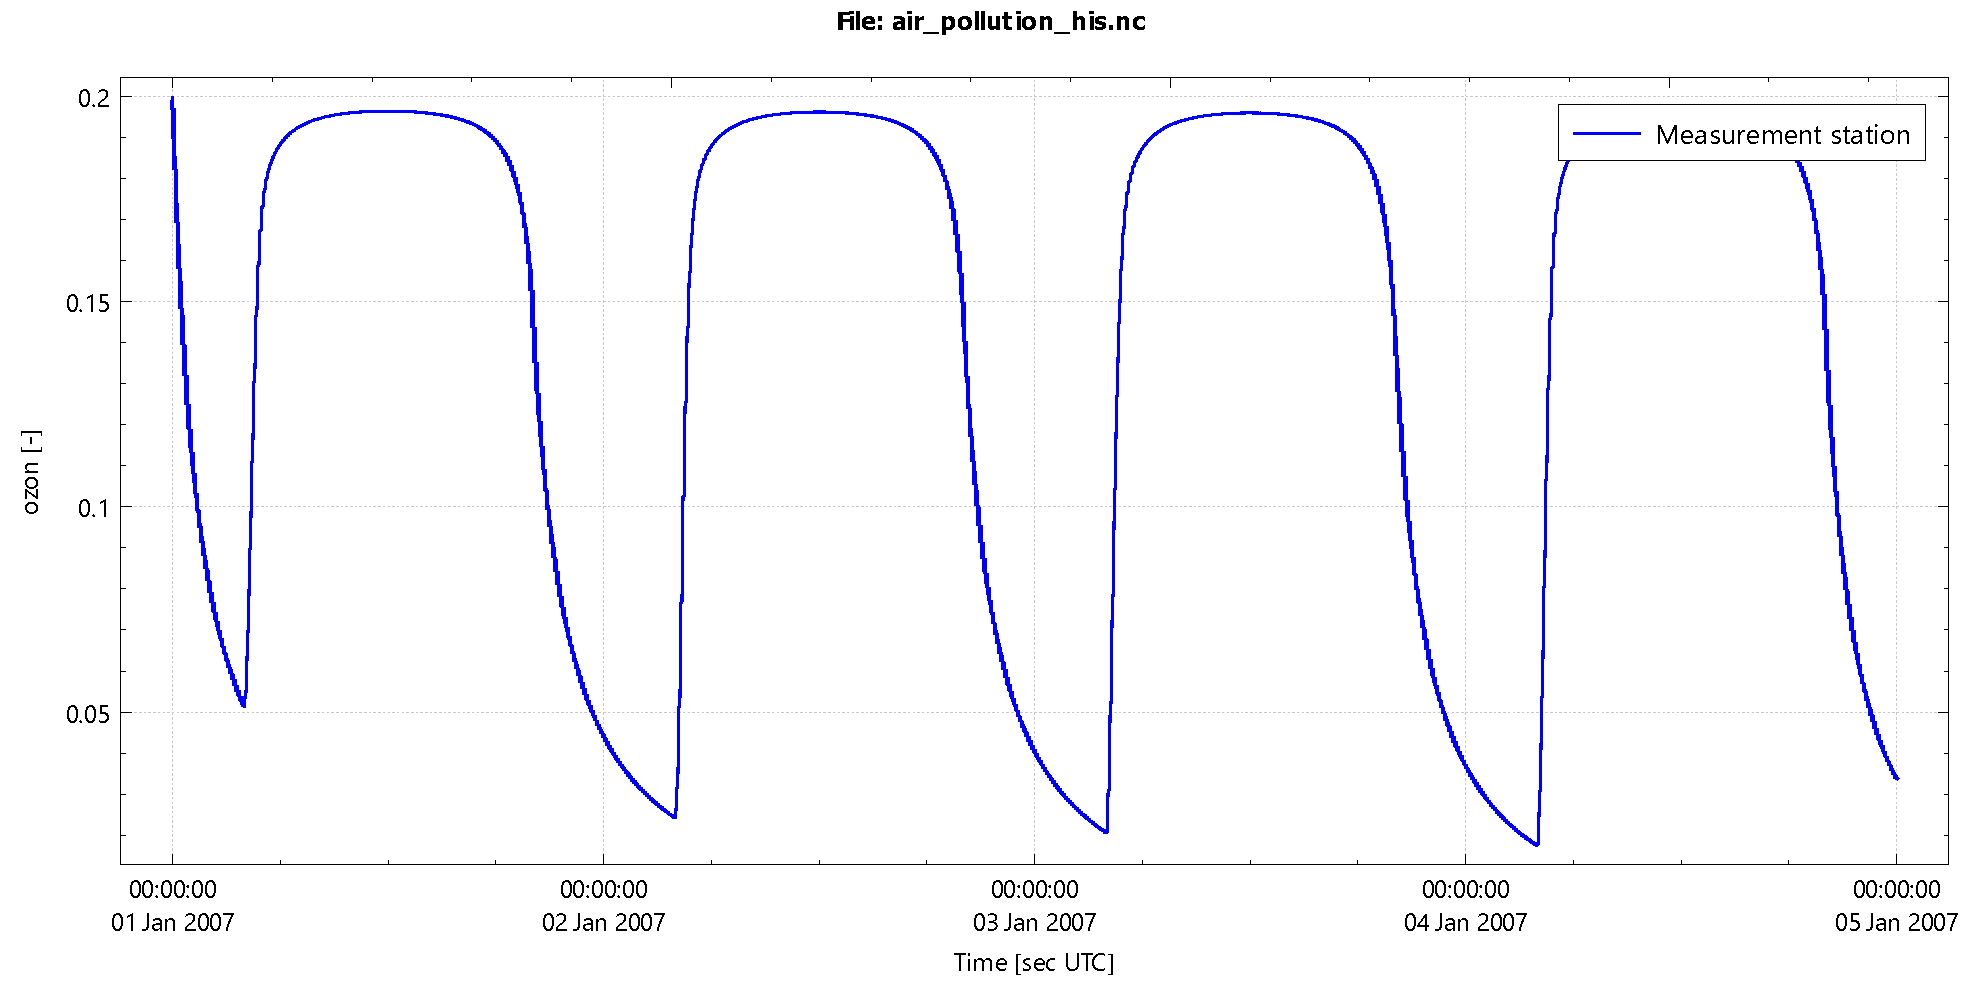
\includegraphics[width=\textwidth]{figures/ozon_dt0d5.pdf}
        \caption{Concentration of Ozon.}
    \end{subfigure}
    \caption[Air pollution experiment: $O$, $N_2$, $NO$ and $O_3$]{Result plots of the different constituents, compute with the fully implicit time integration method with a time step of \bqty{0.5}{\second}.}
\end{figure}

%------------------------------------------------------------------------------
\paragraph*{Different time integrators}
Numerical stability for different values of $\Dt$ are studied for Euler-explicit, Runga-Kutta-4 and the fully implicit $\Delta$-formulation.
%
\begin{longtable}{|>{\bfseries}p{6mm-12pt}|p{\textwidth/4-2mm-12pt}|p{\textwidth/4-2mm-12pt}|p{\textwidth/4-2mm-12pt}|p{\textwidth/4-2mm-12pt}|}
    \caption{Stability for different time integrators} \\%
    \rowcolor{mgreen1}
    & \textcolor{white}{\textbf{Time step\newline \bunit{\second}}}
    & \textcolor{white}{\textbf{Euler explicit}}
    & \textcolor{white}{\textbf{Runge-Kutta 4}}
    & \textcolor{white}{\textbf{Fully Implicit\newline \deltaformulation}}
    \\
    \topline
    \endfirsthead
    \rowcolor{mgreen1}
    & \textcolor{white}{\textbf{Time step\newline \bunit{\second}}}
    & \textcolor{white}{\textbf{Euler Explicit}}
    & \textcolor{white}{\textbf{Runge-Kutta 4}}
    & \textcolor{white}{\textbf{Fully Implicit\newline \deltaformulation}}
    \\
    \midline
    \endhead
    \endfoot
    \bottomline
    \endlastfoot
    1 & 0.5 & -  & \checkmark & \checkmark  \\
    \midline
    2 & 60 & \checkmark  & \checkmark  &  \checkmark \\
    \midline
    3 & 120 & Unstable & \checkmark &  \checkmark \\
    \midline
    4 & 180 & - & Unstable & \checkmark \\
    \midline
    5 & 240 & - & - & \checkmark \\
    \midline
    6 & 300 & - & - & \checkmark \\
    \midline
    7 & 900 & - & - & \checkmark \\
    \midline
    8 & 1800 & - & - & \checkmark \\
    \midline
    9 & 3600 & - & - & \checkmark \\
\end{longtable}

%
%------------------------------------------------------------------------------
\subsection{Brusselator}
%--------------------------------------------------------------------------------
Some numerical results of the brusselator example (\autoref{sec:brusselator}) is:
\begin{figure}[H]
    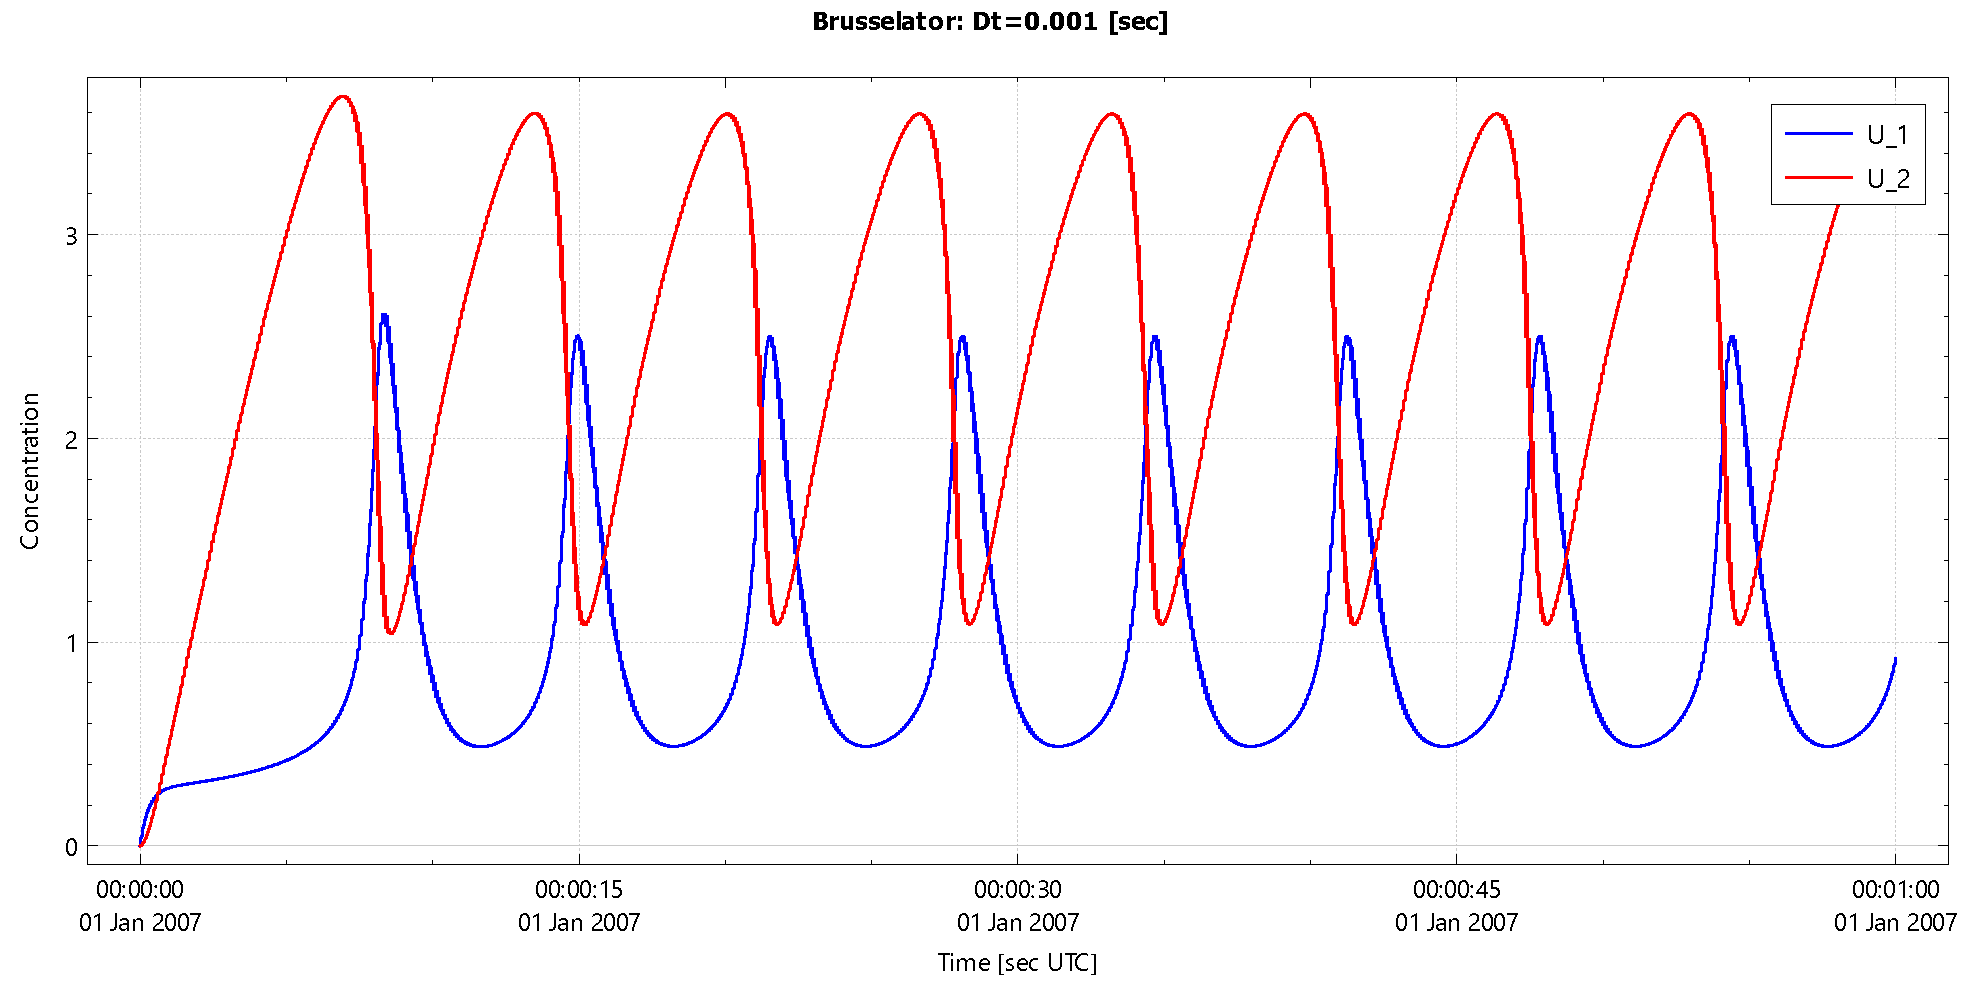
\includegraphics[width=\textwidth]{figures/brusselator_imp_dt=0d001.pdf}
    \caption[Brusselator experiment: $\Dt = 0.001\ \bunit{\second}$]{Fully Implicit: $\Dt=0.001$\ \bunit{\second}, $k_1=1$, $k_2=2.5$. }\label{fig:brusselator_reference}
\end{figure}
The solution presented in \autoref{fig:brusselator_reference} is assumed to be the reference (analytic) solution of \autoref{eq:brusselator}.
%
\begin{figure}[H]
    \begin{subfigure}{0.5\textwidth}
        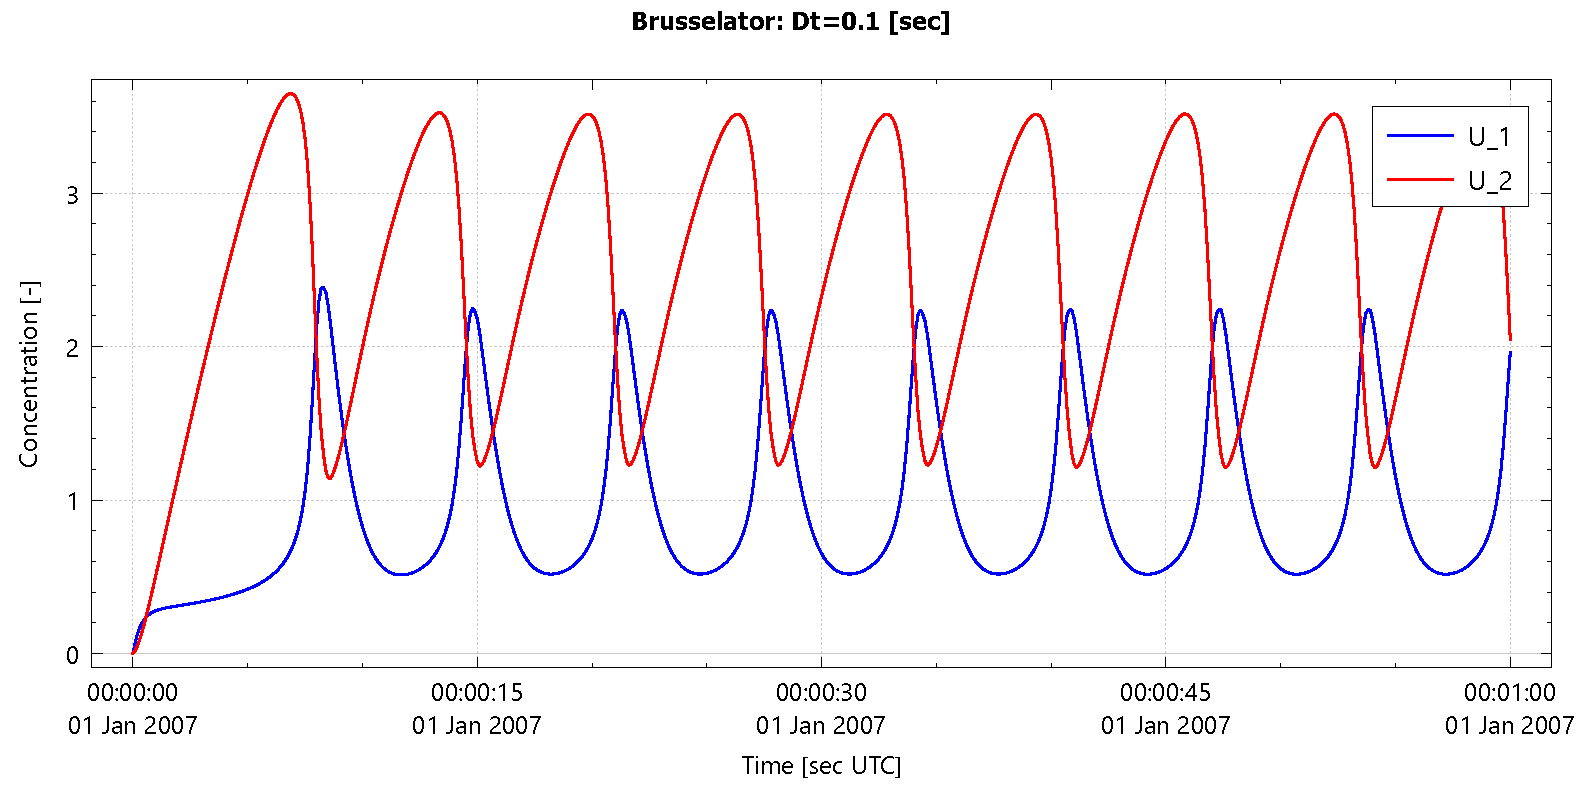
\includegraphics[width=\textwidth]{figures/brusselator_imp_dt=0d10.pdf}
        \caption{Fully Implicit: $\Dt=\bqty{0.1}{\second}$, $k_1=1$, $k_2=2.5$}
    \end{subfigure}
    \begin{subfigure}{0.5\textwidth}
        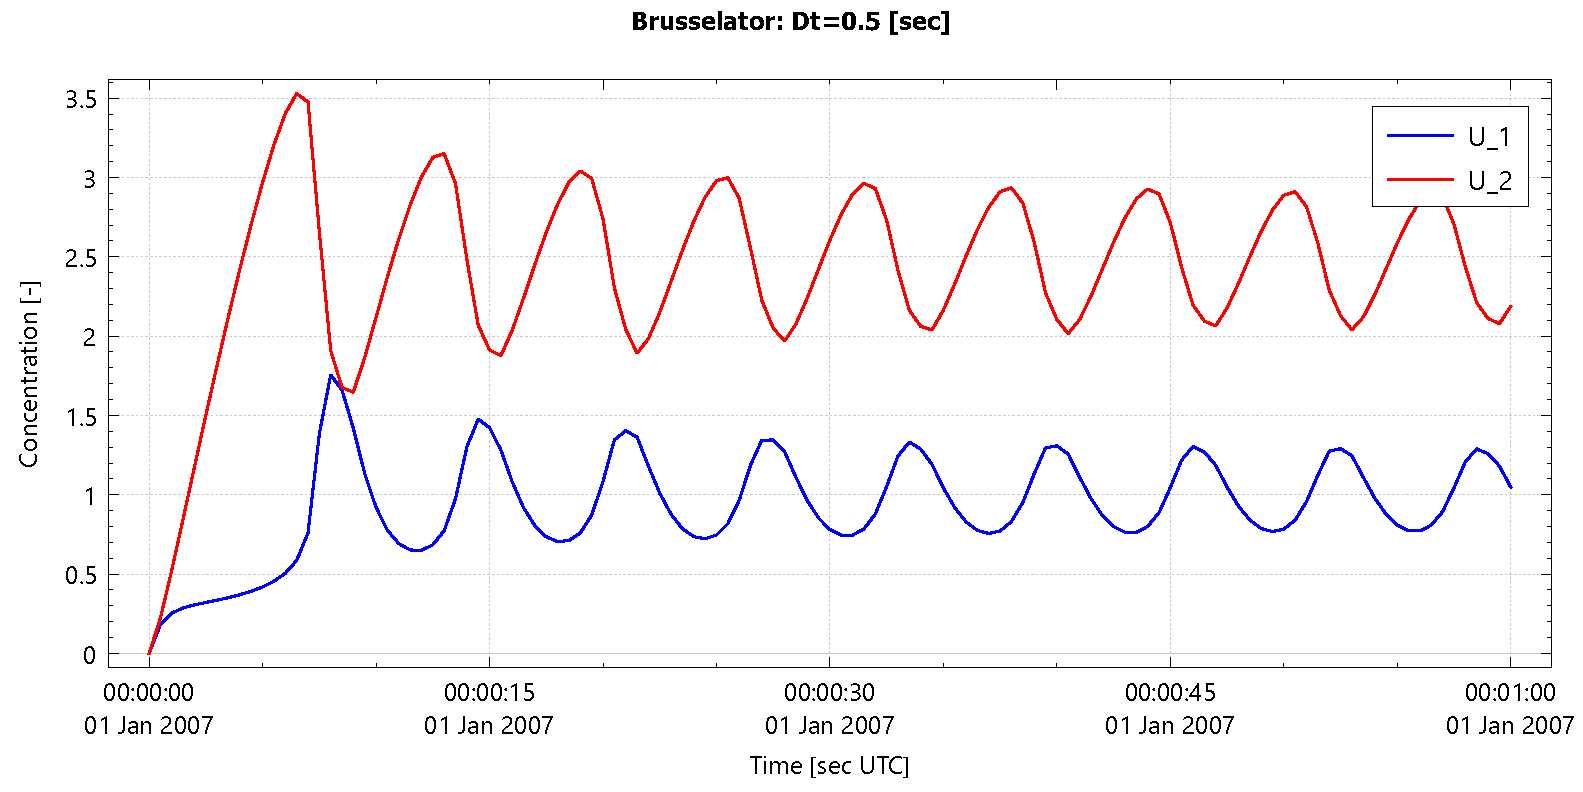
\includegraphics[width=\textwidth]{figures/brusselator_imp_dt=0d50.pdf}
        \caption{Fully Implicit: $\Dt=\bqty{0.5}{\second}$, $k_1=1$, $k_2=2.5$}
    \end{subfigure}
    \caption[Brusselator experiment: $\Dt = 0.1, 0.5\ \bunit{\second}$]{Result plots for constant value of $k_1 = 1$ and $k_2 =2.5$, computed with a fully implicit ($\Delta$ formulation) time integration method for different time steps $\Dt = 0.1, 0.5\ \bunit{\second}$.}
\end{figure}
Extra attention is needed for the Fully Implicit time integration with larger time step:
\begin{figure}[H]
    \begin{subfigure}{0.5\textwidth}
        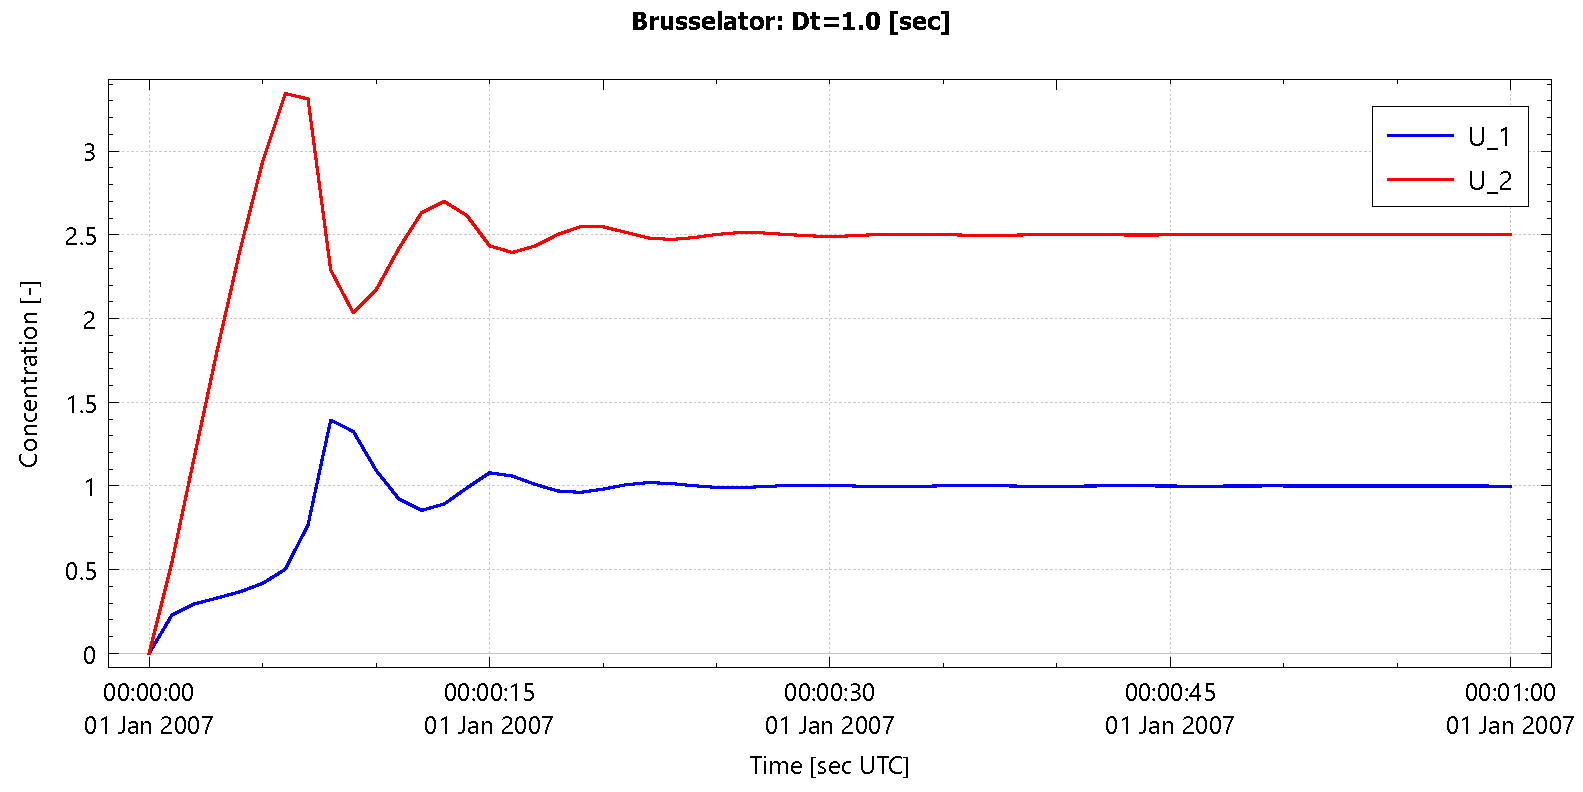
\includegraphics[width=\textwidth]{figures/brusselator_imp_dt=1d00.pdf}
        \caption{Fully Implicit: $\Dt=\bqty{1.0}{\second}$, $k_1=1$, $k_2=2.5$}\label{fig:imp_dt=1d00}
    \end{subfigure}
    \begin{subfigure}{0.5\textwidth}
        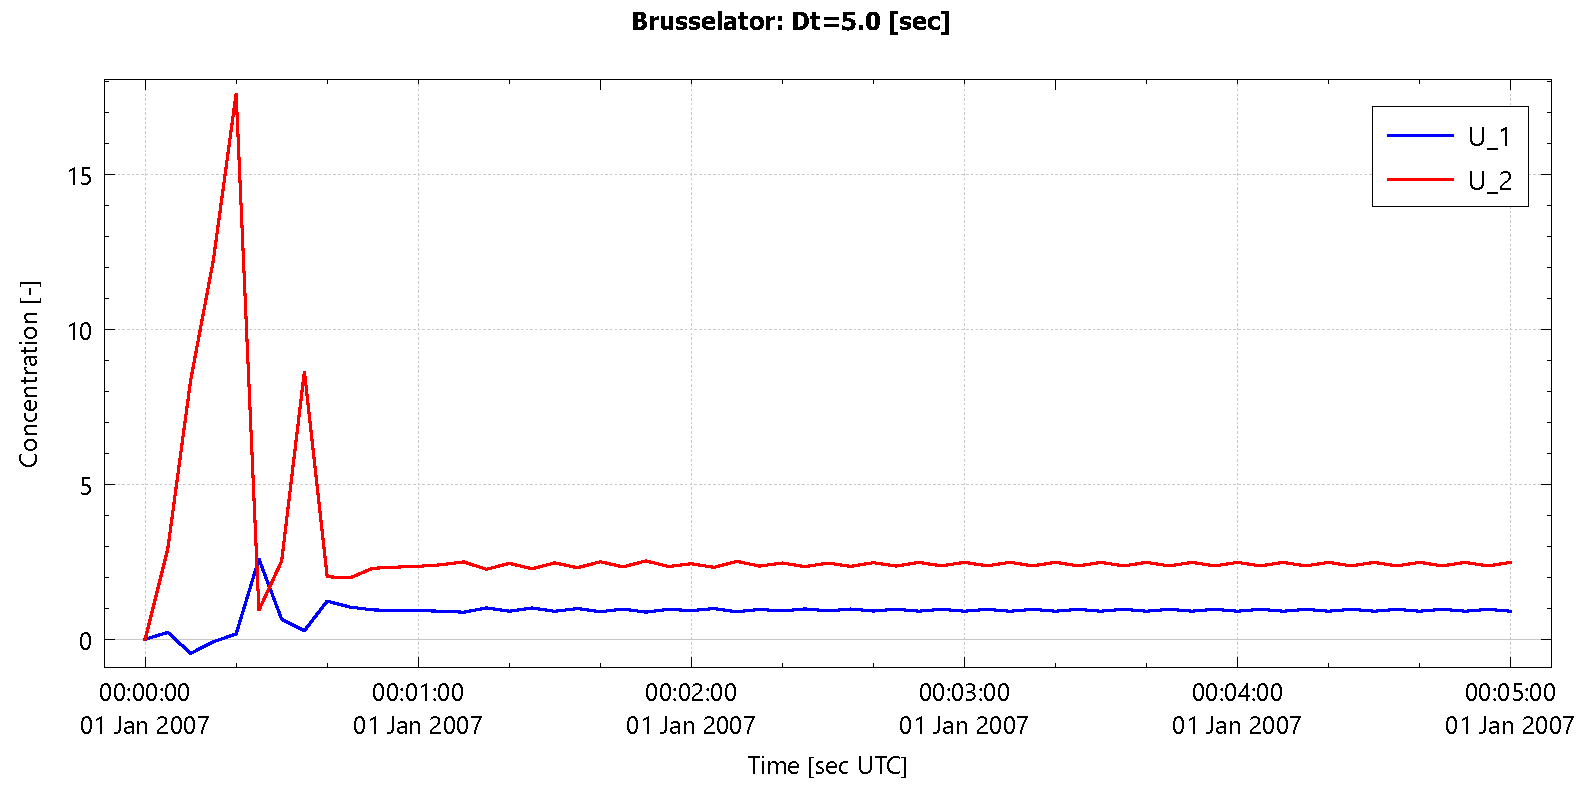
\includegraphics[width=\textwidth]{figures/brusselator_imp_dt=5d00.pdf}
        \caption{Fully Implicit: $\Dt=\bqty{5.0}{\second}$, $k_1=1$, $k_2=2.5$}\label{fig:imp_dt=5d00}
    \end{subfigure}
    \caption[Brusselator experiment: $\Dt = 1.0, 5.0\ \bunit{\second}$]{Result plots for constant value of $k_1 = 1$ and $k_2 =2.5$, computed with a fully implicit ($\Delta$ formulation) time integration method for different time steps $\Dt = 1.0, 5.0\ \bunit{\second}$.
    }
\end{figure}
\Autoref{fig:imp_dt=1d00} converge to the equilibrium state $(u_1, u_2) = (1.0, 2.5)$ and
\Autoref{fig:imp_dt=5d00} looks to converge to the equilibrium state $(u_1, u_2) = (1.0, 2.5)$ but is still wiggling after \bqty{5}{\minute} of simulation time (even after one day --- not presented here).
How these equations are discretized is given in \autoref{sec:brusselator_discretization}.

%------------------------------------------------------------------------------
\paragraph*{Different time integrators}
Numerical stability for different values of $\Dt$ are studied for the Runga-Kutta-4 and fully implicit \deltaformulation.
%
\begin{longtable}{|>{\bfseries}p{6mm-12pt}|p{\textwidth/3-2mm-12pt}|p{\textwidth/3-2mm-12pt}|p{\textwidth/3-2mm-12pt}|}
    \caption{Stability of different time integrators for the Brusselator.} \\%
    \rowcolor{mgreen1}
    & \textcolor{white}{\textbf{Time step\newline \bunit{\second}}}
    & \textcolor{white}{\textbf{Runge-Kutta 4}}
    & \textcolor{white}{\textbf{Fully Implicit\newline \deltaformulation}}
    \\
    \topline
    \endfirsthead
    \rowcolor{mgreen1}
    & \textcolor{white}{\textbf{Time step\newline \bunit{\second}}}
    & \textcolor{white}{\textbf{Runge-Kutta 4}}
    & \textcolor{white}{\textbf{Fully Implicit\newline \deltaformulation}}
    \\
    \midline
    \endhead
    \endfoot
    \bottomline
    \endlastfoot
    1 & 0.1 & \checkmark & \checkmark  \\
    \midline
    2 & 0.2  & \checkmark &  \checkmark   \\
    \midline
    3 & 0.5 & \checkmark &  \checkmark   \\
    \midline
    4 & 1.0 & Unstable &   \checkmark  \\
    \midline
    5 & 2.0 &   &   \checkmark  \\
    \midline
    6 & 5.0 &   &   \checkmark  \\
    \midline
\end{longtable}


%--------------------------------------------------------------------------------
\section{1-D Advection equation}
The considered advection equation reads:
\begin{align}
    \pdiff{c}{t} + \pdiff{uc}{x} = 0,
\end{align}
With a velocity of $u = \bqty{10}{\metre\per\second}$, which coincide with the wave celerity of the 1D-wave numerical experiments as described in \autoref{sec:numerical_experiment}.
\begin{align}
    u(x,t) = \bqty{10}{\metre\per\second}
\end{align}
and with a prescribed boundary condition at the left side of the domain
\begin{align}
    c(0,t) = f_c(t).
\end{align}
%--------------------------------------------------------------------------------
\subsection{Transport of a constant constituent at the boundary} \label{sec:numerical_experiment_1d_adv_constant_boundary}
The prescribed boundary condition for the constituent reads
% reg_factor = 0.5 * (std::cos(M_PI * (treg - double(nst) * dt) / treg) + 1.0);
\begin{align}
    c(0,t) = c_{\it given}
    \begin{cases}
        \half \left(\cos\left(\pi \frac{t_{reg} - t}{t_{reg}} \right) + 1\right) &\quad \text{if } t < t_{reg},
        \\
        1 &\quad \text{if } t \geq t_{reg},
    \end{cases}
    \label{eq:1d_adv_boundary_condition}
\end{align}
where
\begin{symbollist}
    \item[$t_{reg}$] The regularization time for the given time-series, [\si{\second}]
    \nomenclature{$t_{reg}$}{\si{\second}}{The regularization time for the given time-series}
\end{symbollist}
%--------------------------------------------------------------------------------
\paragraph*{Numerical experiment}
The numerical experiment is performed with the following parameters:
\begin{itemize}
    \item Length of the domain, $L_x = \bqty{12000}{\metre}$
    \item Grid size, $\Dx = \bqty{10}{\metre}$
    \item Start time, $t_{start} = \bqty{0}{\second}$
    \item End time, $t_{stop} = \bqty{3600}{\second}$
    \item Timestep, $\Dt = \bqty{5}{\second}$
    \item Regularization time for time-series, $t_{reg} = \bqty{600}{\second}$
    \item Prescribed constant velocity, $u_{\it given}(x,t) = \bqty{10}{\metre\per\second}$
    \item Prescribed initial value of the constituent, $c(x,0)= \bqty{0}{-}$.
    \item Prescribed constituent on boundary at $x=0$ is given by \autoref{eq:1d_adv_boundary_condition}.
    \item No boundary is prescribed at $x=\bqty{12000}{\metre}$.
\end{itemize}
%--------------------------------------------------------------------------------
\paragraph*{Results of the numerical experiments}
A map picture at $t=\bqty{3600}{\second}$ and time-series are given for this experiment.
As seen from the map figure there are very small spurious waves traveling from right to left.
These spurious waves are fully generated by the numerical scheme at the right boundary,
because the continuous advection equation does \textbf{not} allow information traveling from right to left.
\begin{figure}[H]
    \centering
    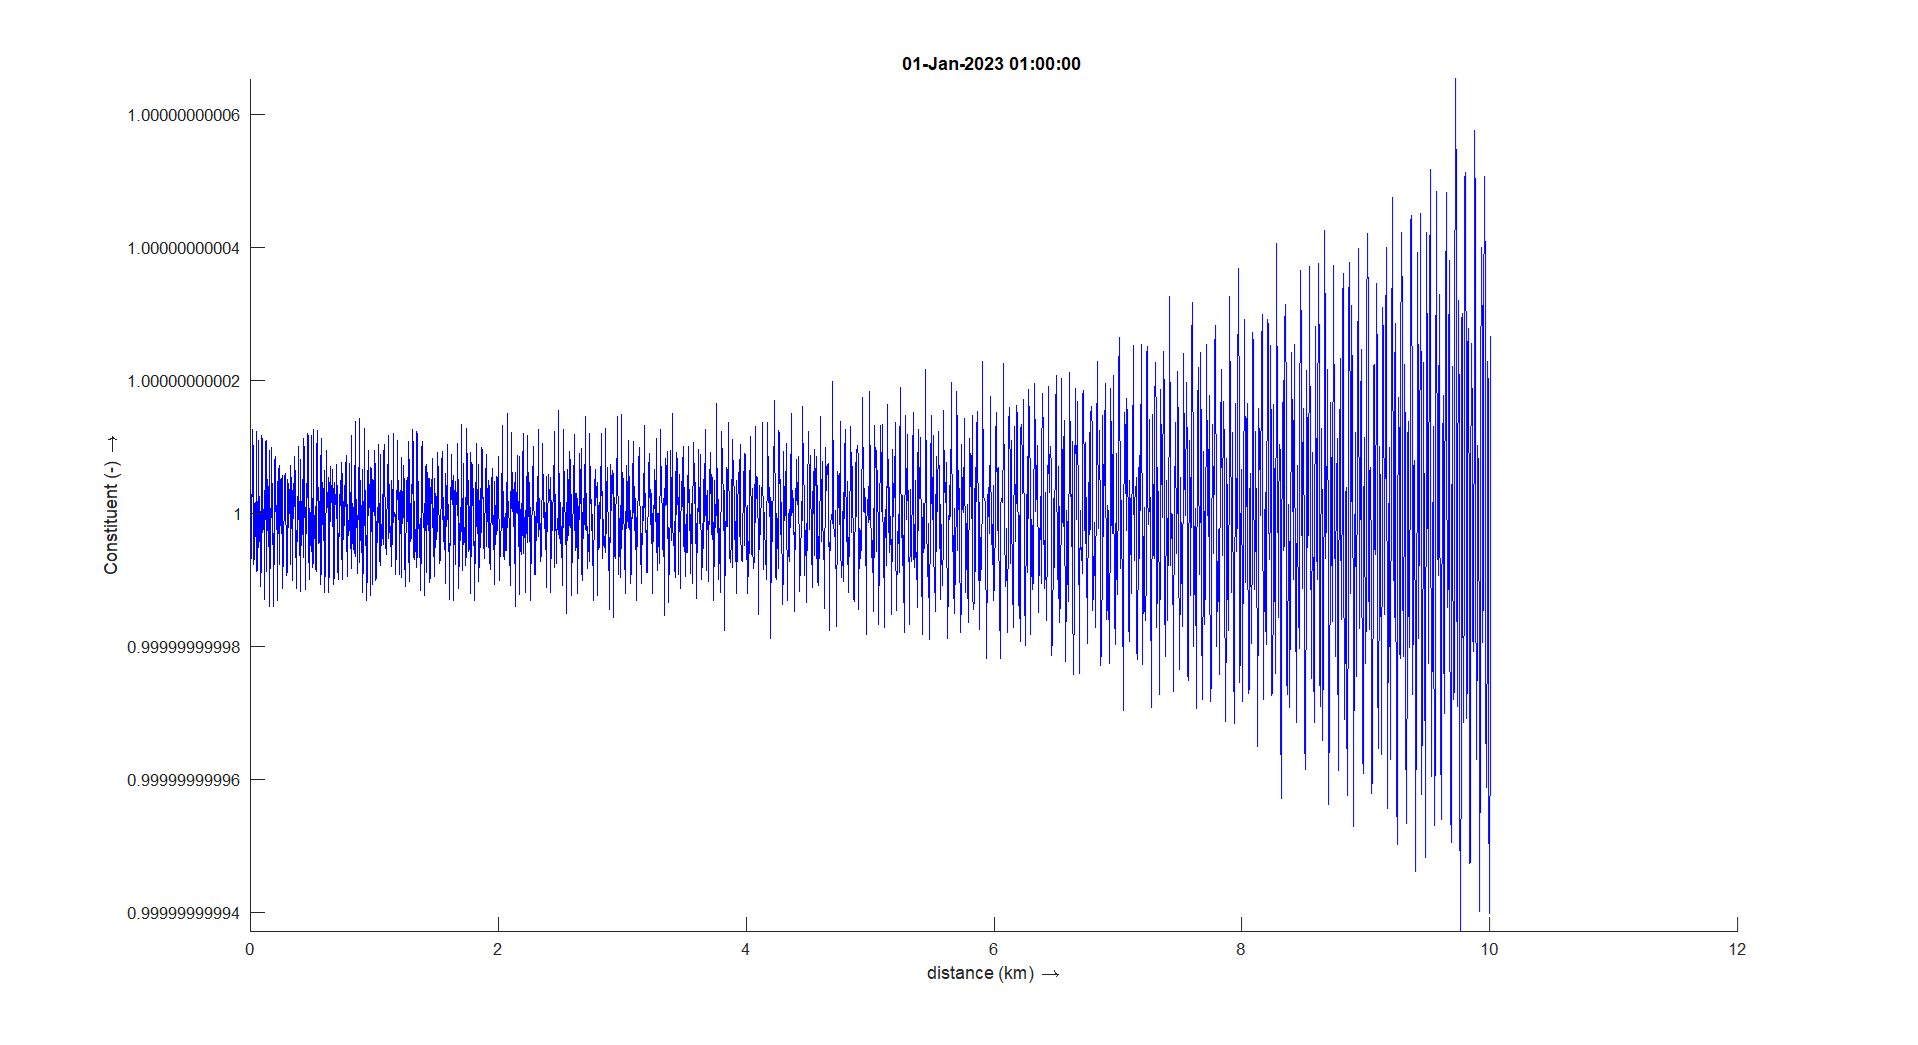
\includegraphics[width=0.9\textwidth]{figures/constant_3600s.png}
    \caption{Spurious waves at $t=\bqty{3600}{\second}$. Range from $ 1 \pm \num{8e-09}$.}
\end{figure}
Results for several observation stations along the channel are shown in \autoref{fig:result_1d_adv_constant_bc}
\begin{figure}[H]
    \centering
    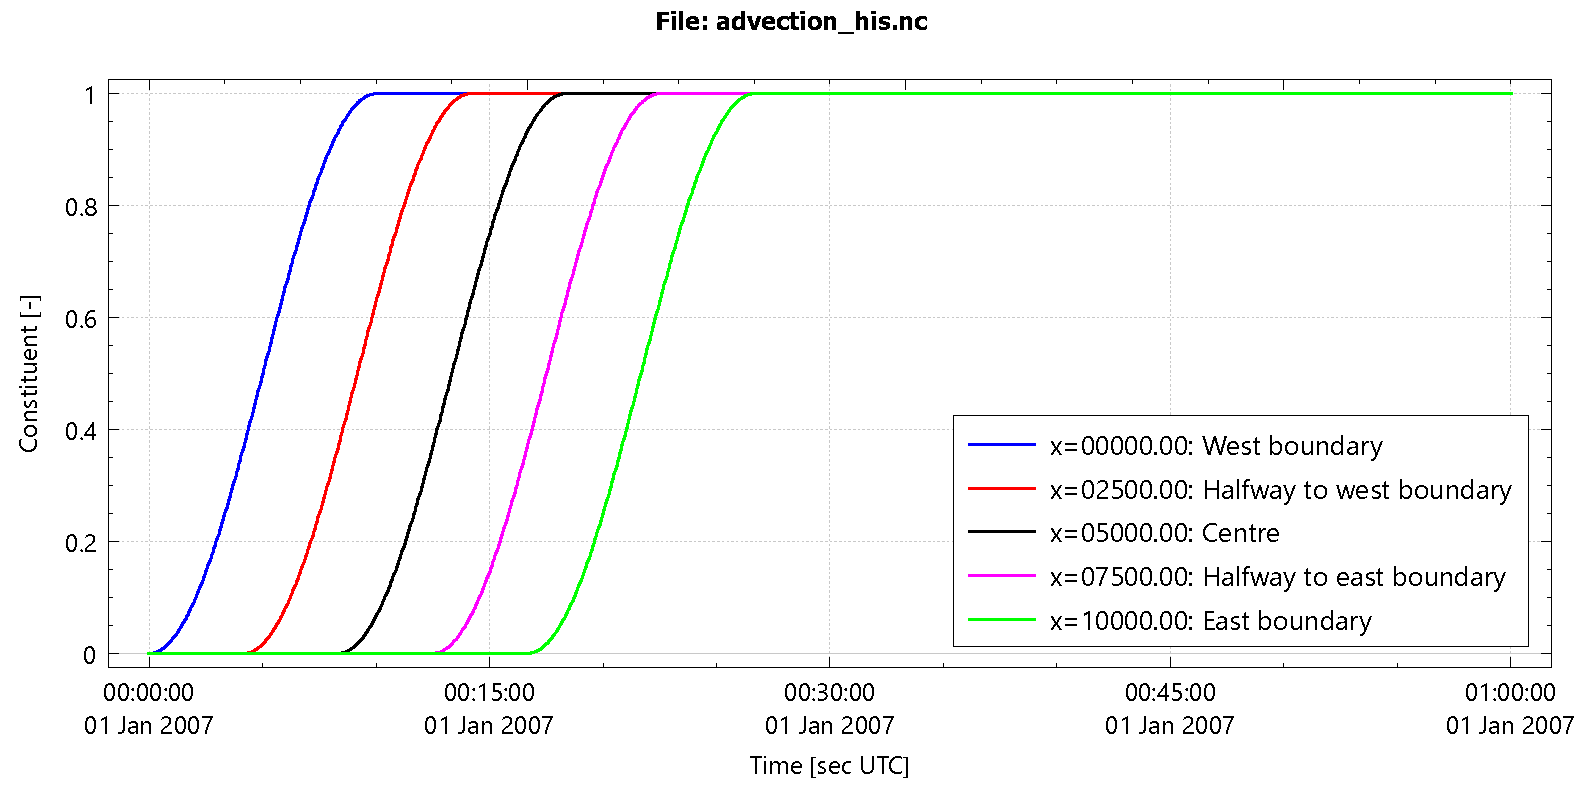
\includegraphics[width=0.9\textwidth]{figures/time-series-advection-constant.pdf}
    \caption{Time-series for several stations in the model, showing the transition behavior between the initial situation and the time-independent solution.}
    \label{fig:result_1d_adv_constant_bc}
\end{figure}
%--------------------------------------------------------------------------------
\subsection{Transport of a time-dependent constituent at the boundary}
\label{sec:numerical_experiment_1d_adv_time_dependent_boundary}
The prescribed boundary condition for the constituent reads
% reg_factor = 0.5 * (std::cos(M_PI * (treg - double(nst) * dt) / treg) + 1.0);
\begin{align}
    c(0,t) = c_{\it given}
    \begin{cases}
        \half \left(\cos\left(\pi \frac{t_{reg} - t}{t_{reg}}\right) + 1  \right) &\quad \text{if } t < t_{reg},
        \\
        -\cos\left(\pi \frac{t}{t_{\it reg}} \right) &\quad \text{if } t \geq t_{reg},
    \end{cases}
    \label{eq:1d_adv_sine_boundary_condition}
\end{align}
where
\begin{symbollist}
    \item[$t_{reg}$] The regularization time for the given time-series, [\si{\second}]
    \nomenclature{$t_{reg}$}{\si{\second}}{The regularization time for the given time-series}
\end{symbollist}
%--------------------------------------------------------------------------------
\paragraph*{Numerical experiment}
The numerical experiment is performed with the following parameters:
\begin{itemize}
    \item Length of the domain, $\bqty{12000}{\metre}$
    \item Grid size, $\Dx = \bqty{10}{\metre}$
    \item Start time, $t_{start} = \bqty{0}{\second}$
    \item End time, $t_{stop} = \bqty{3600}{\second}$
    \item Timestep, $\Dt = \bqty{10}{\second}$
    \item Regularization time for time-series, $t_{reg} = \bqty{600}{\second}$
    \item Prescribed constant velocity, $u_{\it given}(x,t) = \bqty{10}{\metre\per\second}$
    \item Prescribed initial value of the constituent, $c(x,0)= \bqty{0}{-}$.
    \item Prescribed constituent on boundary at $x=0$ is given by \autoref{eq:1d_adv_boundary_condition}.
    \item No boundary is prescribed at $x=\bqty{12000}{\metre}$.
\end{itemize}
%--------------------------------------------------------------------------------
\paragraph*{Results of the numerical experiments}
Results for several observation stations along the channel are shown in  \autoref{fig:result_1d_adv_sine_bc}:
\begin{figure}[H]
    \centering
    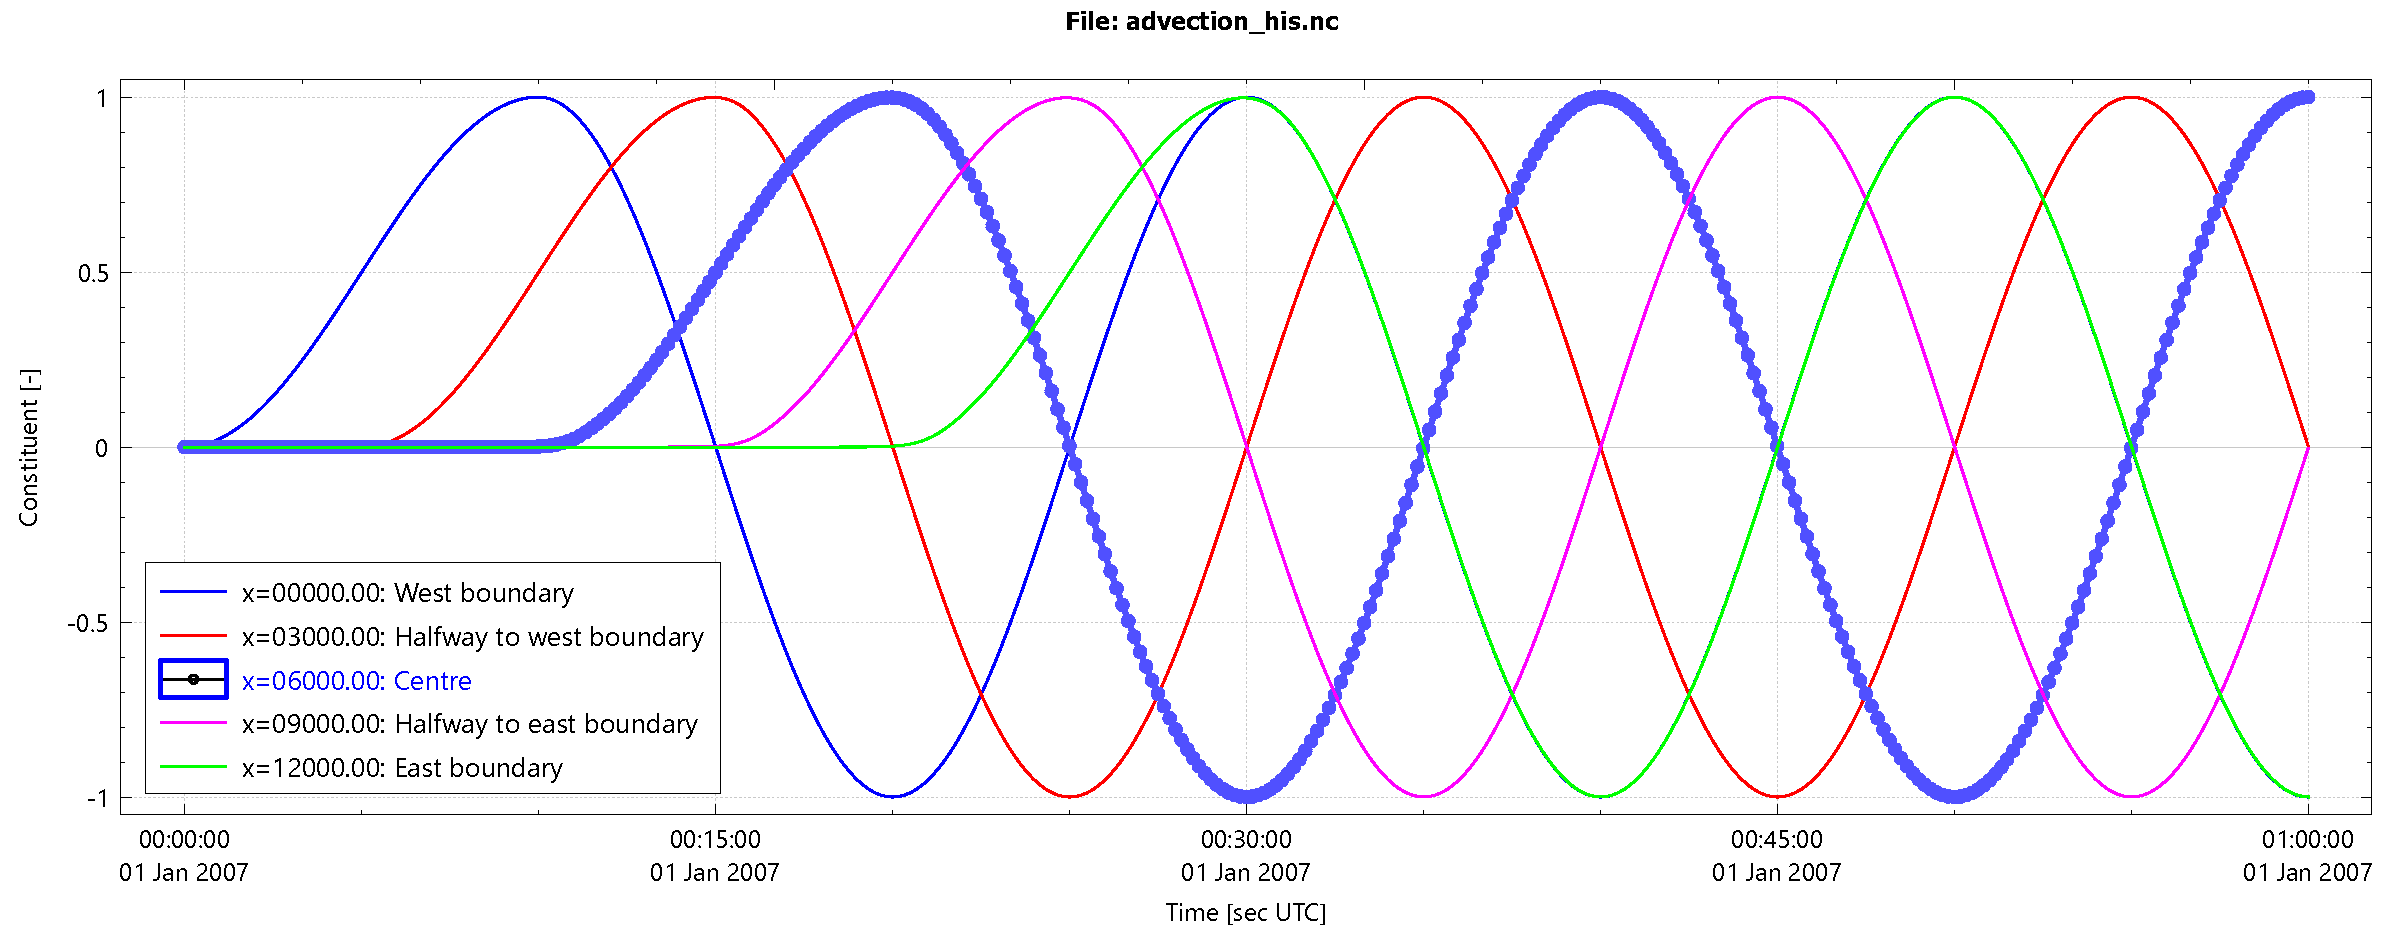
\includegraphics[width=0.9\textwidth]{figures/1d_advec_sine_dx10d0.pdf}
    \caption{Time-series for several stations in the model, showing the transition behavior between the initial situation and the time-independent solution.}
    \label{fig:result_1d_adv_sine_bc}
\end{figure}
%--------------------------------------------------------------------------------
\subsection{Transport of a wave package inside the domain}
The initial condition are computed as described in \autoref{sec:compatible_initialization}
and is illustrated in \autoref{fig:1d_adv_initial_wave_package}:
\begin{figure}[H]
    \centering
    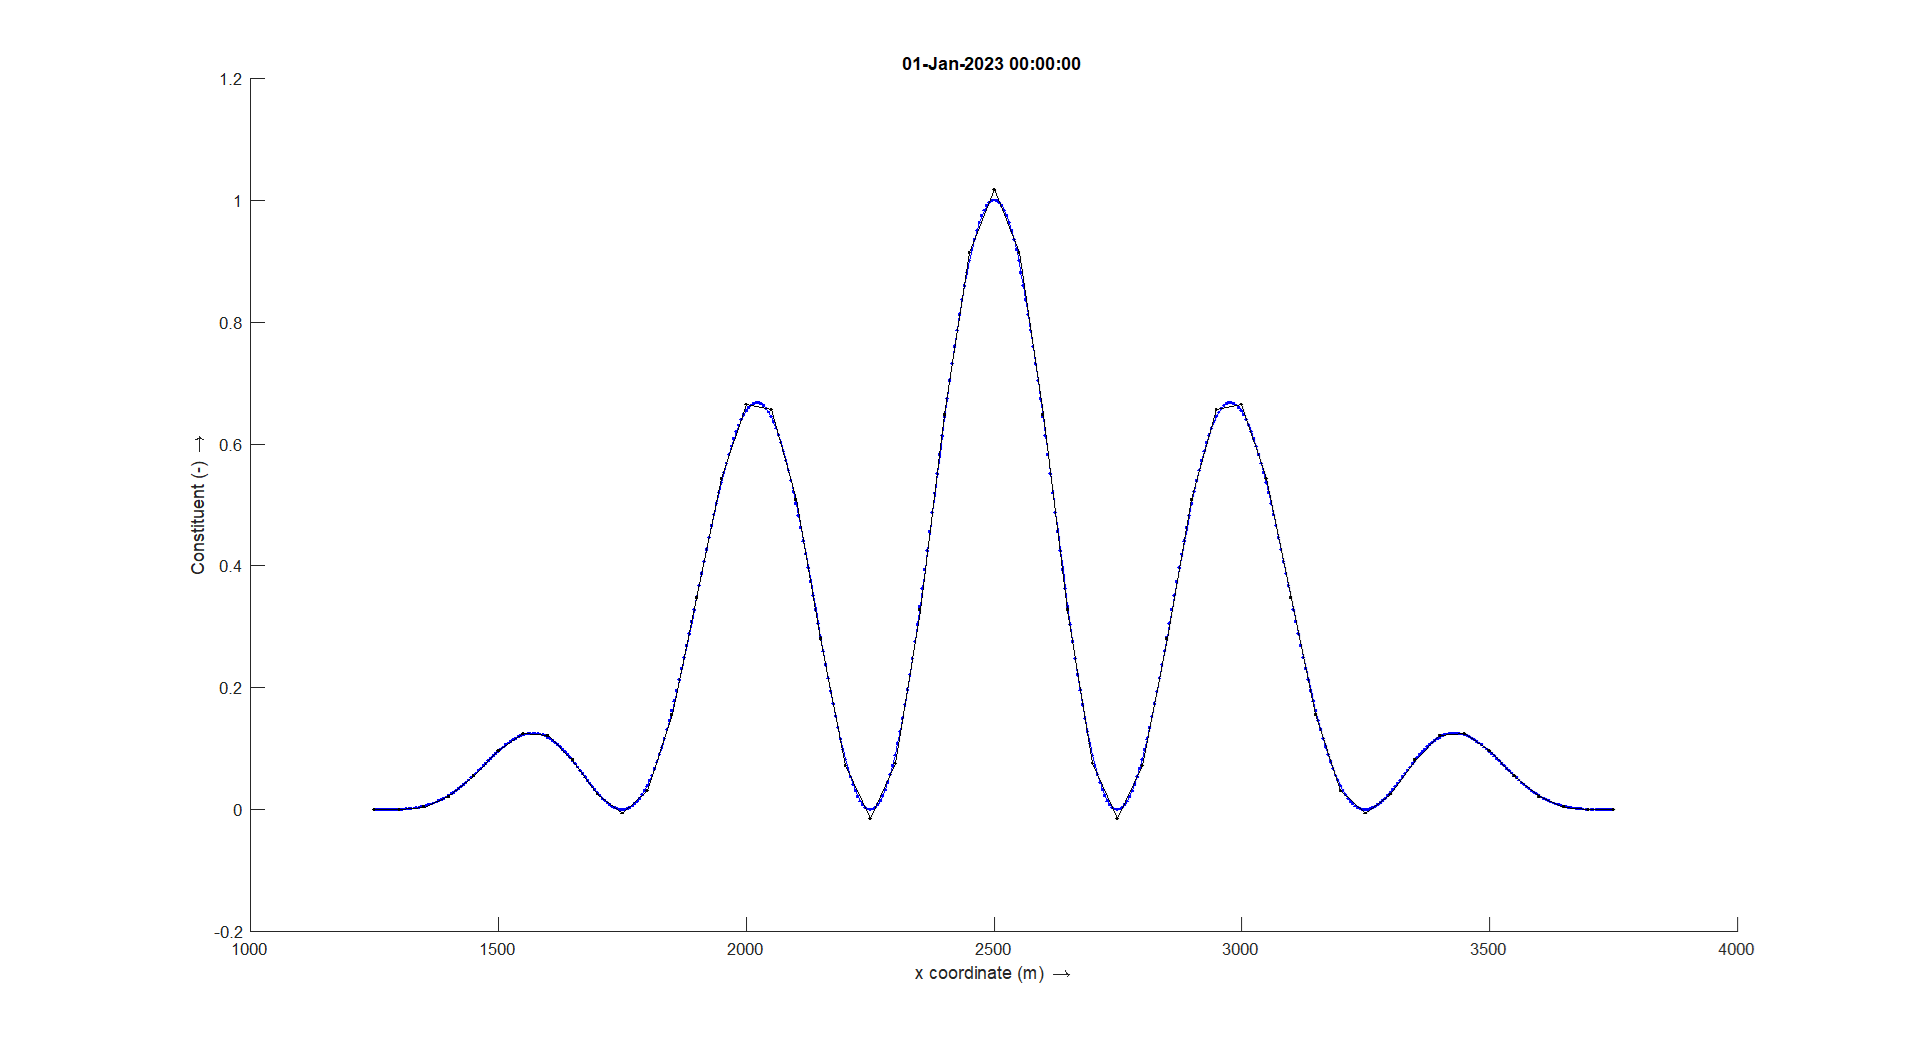
\includegraphics[width=0.9\textwidth]{figures/wave_package_000s.png}
    \caption{Compatible initial condition of the wave package. Blue: Initial condition when  $\Dx=\bqty{5}{\metre}$, Black: Initial condition when  $\Dx=\bqty{50}{\metre}$.}
    \label{fig:1d_adv_initial_wave_package}
\end{figure}
The graphs in \autoref{fig:1d_adv_initial_wave_package} do not coincide on the grid points because the profiles are computed according \autoref{sec:compatible_initialization}.
The initial condition is defined by:
\begin{align}
    u_{it given} =
    \begin{cases}
        0, & 0 < 1250, \bunit{\metre} \\
        \left(\half + \half \cos( 5k_{\it env}(x - x_{\it cent})) \right) \times \\
        \qquad\left(\half + \half \cos( k_{\it env} (x - x_{\it cent})) \right)
        & 1250 < 3750,  \bunit{\metre}
        \\
        0,  & 3750 < 10000,  \bunit{\metre}
    \end{cases}
\end{align}
with
\begin{symbollist}
    \item[$x_{\it cent}$] Location of the centre of the envelope.
    \item[$L_{\it env}$] Length of the envelope.
    \item[$k_{\it env}$] $k_{\it env} = 2\pi / L_{\it env}$.
\end{symbollist}

%--------------------------------------------------------------------------------
\paragraph*{Numerical experiment}
The numerical experiment is performed with the following parameters:
\begin{itemize}
    \item Length of the domain $L_x = \bqty{10000}{\metre}$.
    \item Length of the envelope \bqty{2500}{\metre}, ranging from \bqty{1250}{\metre} to \bqty{3750}{\metre}.
    \item Grid size and time step,
    \begin{itemize}
        \item $\Dx = \bqty{5}{\metre}$ and $\Dt = \bqty{0.01}{s}$
        \item $\Dx = \bqty{10}{\metre}$ and $\Dt = \bqty{0.01}{s}$
        \item $\Dx = \bqty{25}{\metre}$ and $\Dt = \bqty{0.01}{s}$
        \item $\Dx = \bqty{50}{\metre}$ and $\Dt = \bqty{0.01}{s}$
        \item $\Dx = \bqty{100}{\metre}$ and $\Dt = \bqty{0.01}{s}$
    \end{itemize}
    \item Start time, $t_{start} = \bqty{0}{\second}$.
    \item End time, $t_{stop} = \bqty{250}{\second}$.
    \item Prescribed boundary conditions: $c(0,t) = c(L_x,t) = 0$.
    \item \textbf{No} regularization is applied.
\end{itemize}
%--------------------------------------------------------------------------------
\paragraph*{Results of the numerical experiments}
Results for the four different computations are shown in \autoref{fig:result_wave_package}
\begin{figure}[H]
    \centering
    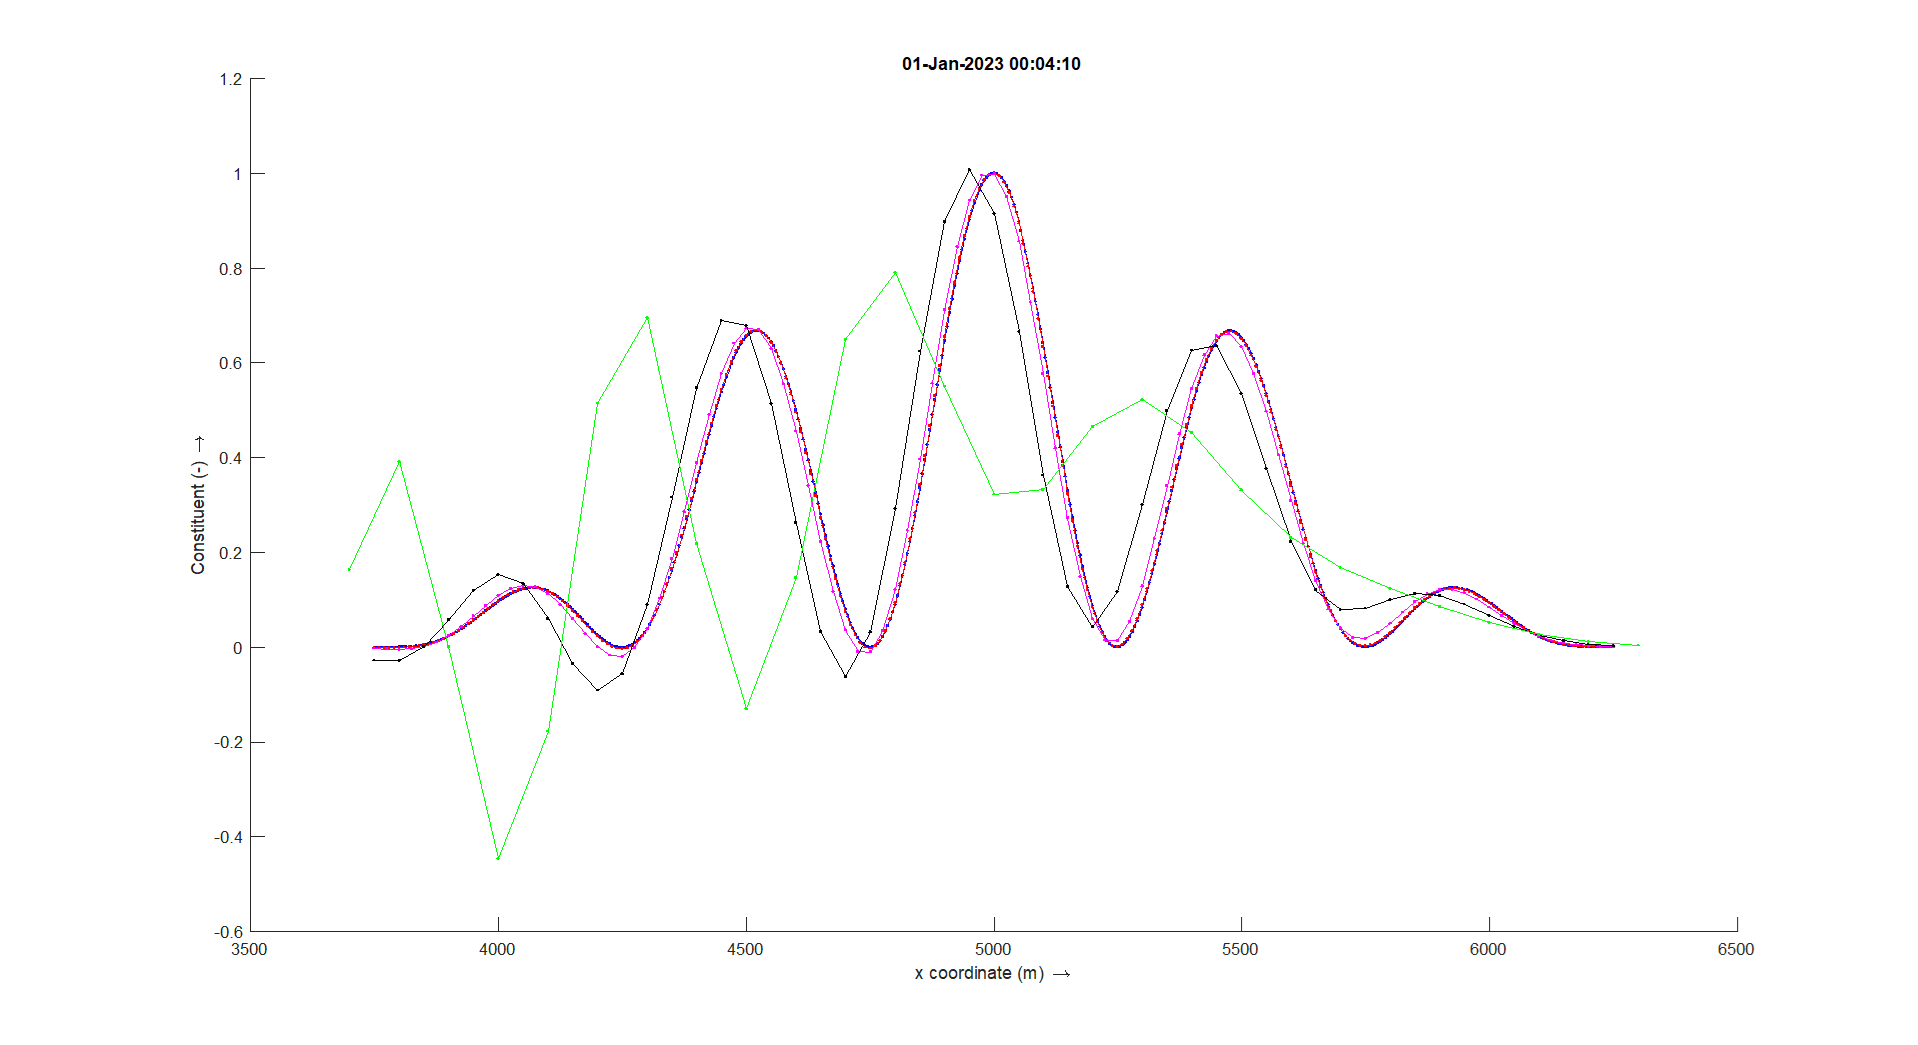
\includegraphics[width=0.9\textwidth]{figures/wave_package_250s.png}
    \caption[Wave package experiment]{Wave package experiment, results at $t=\bqty{250}{\second}$ and $\Dt = \bqty{0.01}{\second}$:
        Blue: $\Dx = \bqty{5}{\metre}$,
        Red: $\Dx = \bqty{10}{\metre}$,
        Cyan: $\Dx = \bqty{25}{\metre}$,
        Black: $\Dx = \bqty{50}{\metre}$,
        Green: $\Dx = \bqty{100}{\metre}$.
    }
    \label{fig:result_wave_package}
\end{figure}


%--------------------------------------------------------------------------------
\subsection{Transport of strictly positive constituent}
When $c$ needs a strickly positive value (like a concentration) then due to numerical discretization the value $c$ could become negative, even if the initial and boundary values are positive.
In certain applications a positive value is required and even small negative are not allowed.
To ensure the positivity of the constituent $c$ we will write the equation with variable $\phi$, where $\phi$ is defined as:
\begin{align}
    c = \exp(\ln(c)) =  \exp(\phi), \quad \text{with} \quad \phi = \ln(c)
\end{align}
The considered advection-diffusion equation than reads:
\begin{align}
    \int_\Omega\pdiff{{e^\phi}}{t} \, d\omega
    + \int_\Omega\pdiff{\left(u{e^\phi}\right)}{x} \, d\omega
    - \int_\Omega\pdiff{}{x}\left(\eps \pdiff{{e^\phi}}{x}\right)\, d\omega = 0,\label{eq:1d_advec_phi_num}
\end{align}
With initial condition for the velocity $u_{\it given} = \bqty{10}{\metre\per\second}$, which coincide with the wave celerity in the next numerical experiments.
\begin{align}
    u(x,0) = u_{\it given}
\end{align}
and with a prescribed boundary condition for the constituent $c$ at the left side of the domain
\begin{align}
    c(0,t) = c_{\it given}
    \begin{cases}
        \half \cos\left(\pi \left(\frac{t_{reg} - t}{t_{reg}}\right)+ 1\right) &\quad \text{if } t < t_{reg},
        \\
        1 &\quad \text{if } t \geq t_{reg},
    \end{cases}
\end{align}
where
\begin{symbollist}
    \item[$t_{reg}$] The regularization time for the given time-series, [\si{\second}]
    \nomenclature{$t_{reg}$}{\si{\second}}{The regularization time for the given time-series}
\end{symbollist}
A value of $c(0,t)=0$ is estimated by:
\begin{align}
    \phi(0,t) = \ln(c(0,t)) \gtrsim -25
\end{align}
%--------------------------------------------------------------------------------
\paragraph*{Numerical experiment}
The numerical experiment is performed with the following parameters:
\begin{itemize}
    \item Length of the domain, $\bqty{12000}{\metre}$
    \item Grid size, $\Dx = \bqty{10}{\metre}$
    \item Start time, $t_{start} = \bqty{0}{\second}$
    \item End time, $t_{stop} = \bqty{3600}{\second}$
    \item Timestep, $\Dt = \bqty{5}{\second}$
    \item Regularization time for time-series, $t_{reg} = \bqty{300}{\second}$
    \item Prescribed constant velocity, $u_{\it given}(x,t) = \bqty{10}{\metre\per\second}$
    \item Prescribed initial value of the constituent, $c(x,0)= \num{1.4e-11}$, \newline so $\phi = \bqty{-25}{-}$.
    \item Prescribed constant constituent on boundary $c_{\it given}(0,t) = 1$, \newline so $\phi = \ln(c_{\it given}(0,t)) = \ln(1) = \bqty{0}{-}$
\end{itemize}
%--------------------------------------------------------------------------------
\paragraph*{Results of the numerical experiments}
\notyet
%--------------------------------------------------------------------------------
\section{1-D Advection-diffusion equation}
In this section we will show the resuls of the advection-diffusion equation with a Dirichlet boundary conditions at both sides of the domain and an interface problem, i.e.\ a large jump of the diffusion coefficiebt in the middle of the domain.

The considered advection-diffusion equation reads:
\begin{align}
    \pdiff{c}{t} + \pdiff{uc}{x} - \pdiff{}{x}\left( (\eps+\Psi) \pdiff{c}{x}\right)= 0, \qquad u>0. \label{eq:1d_advection_art_diff}
\end{align}
where
\begin{symbollist}
    \item[$c$] Constituent, $\bunit{-}$.
    \item[$u$] Advection velocity, $\bunit{\metre\per\second}$.
    \item[$\eps$] Diffusion coefficient, $\bunit{\square\metre\per\second}$.
    \item[$\Psi$] Artificial diffusion, $\bunit{\square\metre\per\second}$.
\end{symbollist}

%--------------------------------------------------------------------------------
\subsection{Outflow boundary layer}\label{sec:1d_numerical_outflow_boundary_layer_experiment}
The Dirichlet value at the outflow boundary is so chosen that there will appear an outflow boundary layer.
Due to this outflow boundary the numerical scheme need to have a cell P\'eclet number ($\Pe = u\Dx/\eps$) smaller then two in the vicinity of that layer.
In the \deltaformulation that will be reach by a regularization step, i.e. increase the diffusion in the vicinity of the boundary layer.
To force a outflow boundary layer at both boundaries a Dirichlet boundary is prescribed.
With the boundary conditions
$c(0,t) = a$ and $c(L,t) = b$ the analytic solution read:
\begin{align}
    c(x) = a + (b-a) \frac{e^{\frac{(x-L)}{L}\Pe} -  e^{-\Pe}}{1 - e^{-\Pe}},
\end{align}
with $\Pe = u L/\eps$.

%--------------------------------------------------------------------------------
\paragraph*{Numerical experiment}
The numerical experiment is performed with the following parameters:
\begin{itemize}
    \item Length of the domain $L_x = \bqty{1000}{\metre}$.
    \item Stationary simulation, $\lpdiff{c}{t}=0$.
    \item Prescribed boundary conditions: $c(0,t) = 0$ and $c(L_x,t) = 1$.
    \item Grid size $\Dx = \bqty{10}{\metre}$,
    \item Diffusion coefficient $\eps = \bqty{10}{\square\metre\per\second}$
    \item Advection velocities, $\Pe = u\Dx/\eps$:
    \begin{itemize}
        \item $u = \bqty{1}{\metre\per\second} \rightarrow \Pe = 1.0$
        \item $u = \bqty{1.9}{\metre\per\second} \rightarrow \Pe = 1.9$
        \item $u = \bqty{2.1}{\metre\per\second} \rightarrow \Pe = 2.1$
        \item $u = \bqty{5.0}{\metre\per\second} \rightarrow \Pe = 5.0$
    \end{itemize}
    \item Smoothing factor, $c_{\Psi} = 4$
    \item Right hand side to compute artificial viscosity, $\frac{1}{32} c_{\Psi} u \Dx \lpdiff[2]{c}{\xi}$ (educational guess).
\end{itemize}
%--------------------------------------------------------------------------------
\paragraph*{Results of the numerical experiments}
Map results are presented for the constituent $c$ and the artificial diffusion $\Psi$.
\begin{figure}[H]
    \begin{subfigure}{0.5\textwidth}
    \centering
    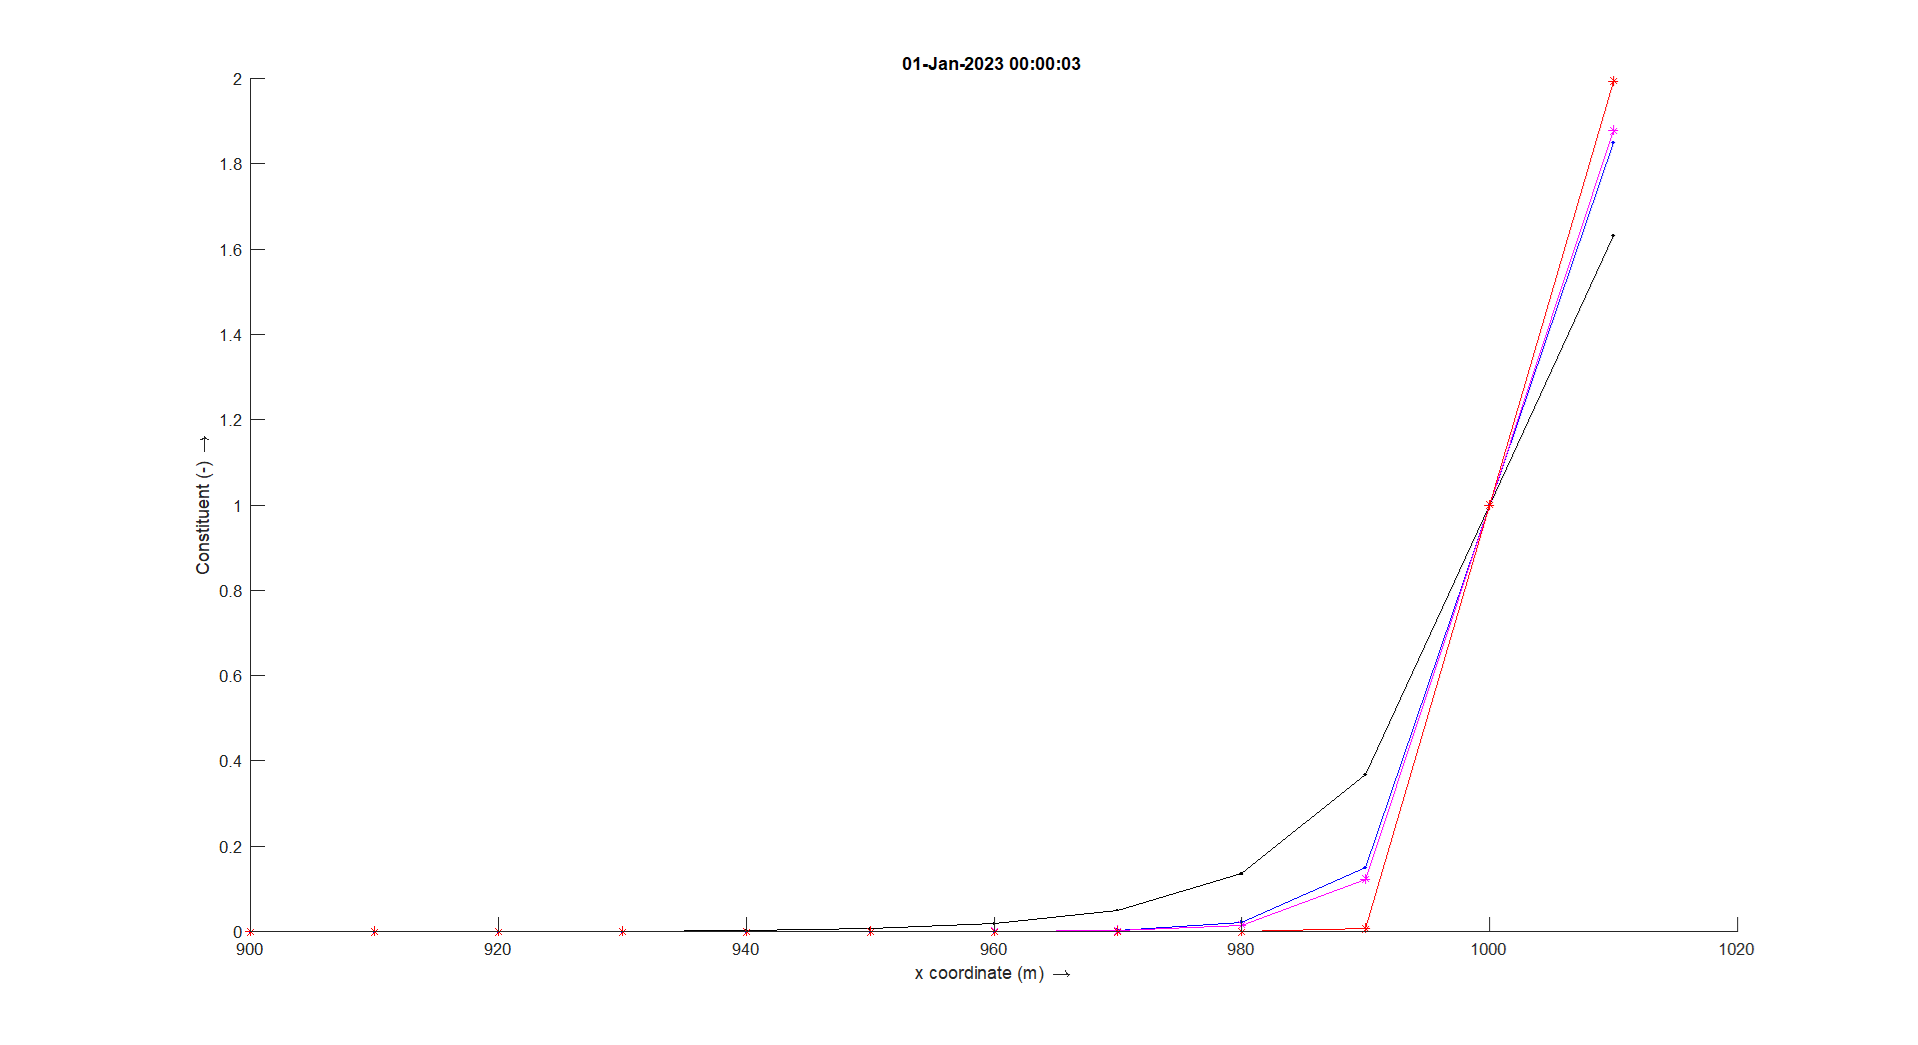
\includegraphics[width=0.9\textwidth]{figures/analytic_boundary_layer.png}
    \caption{Analytic solution}
    \end{subfigure}
    \begin{subfigure}{0.5\textwidth}
    \centering
    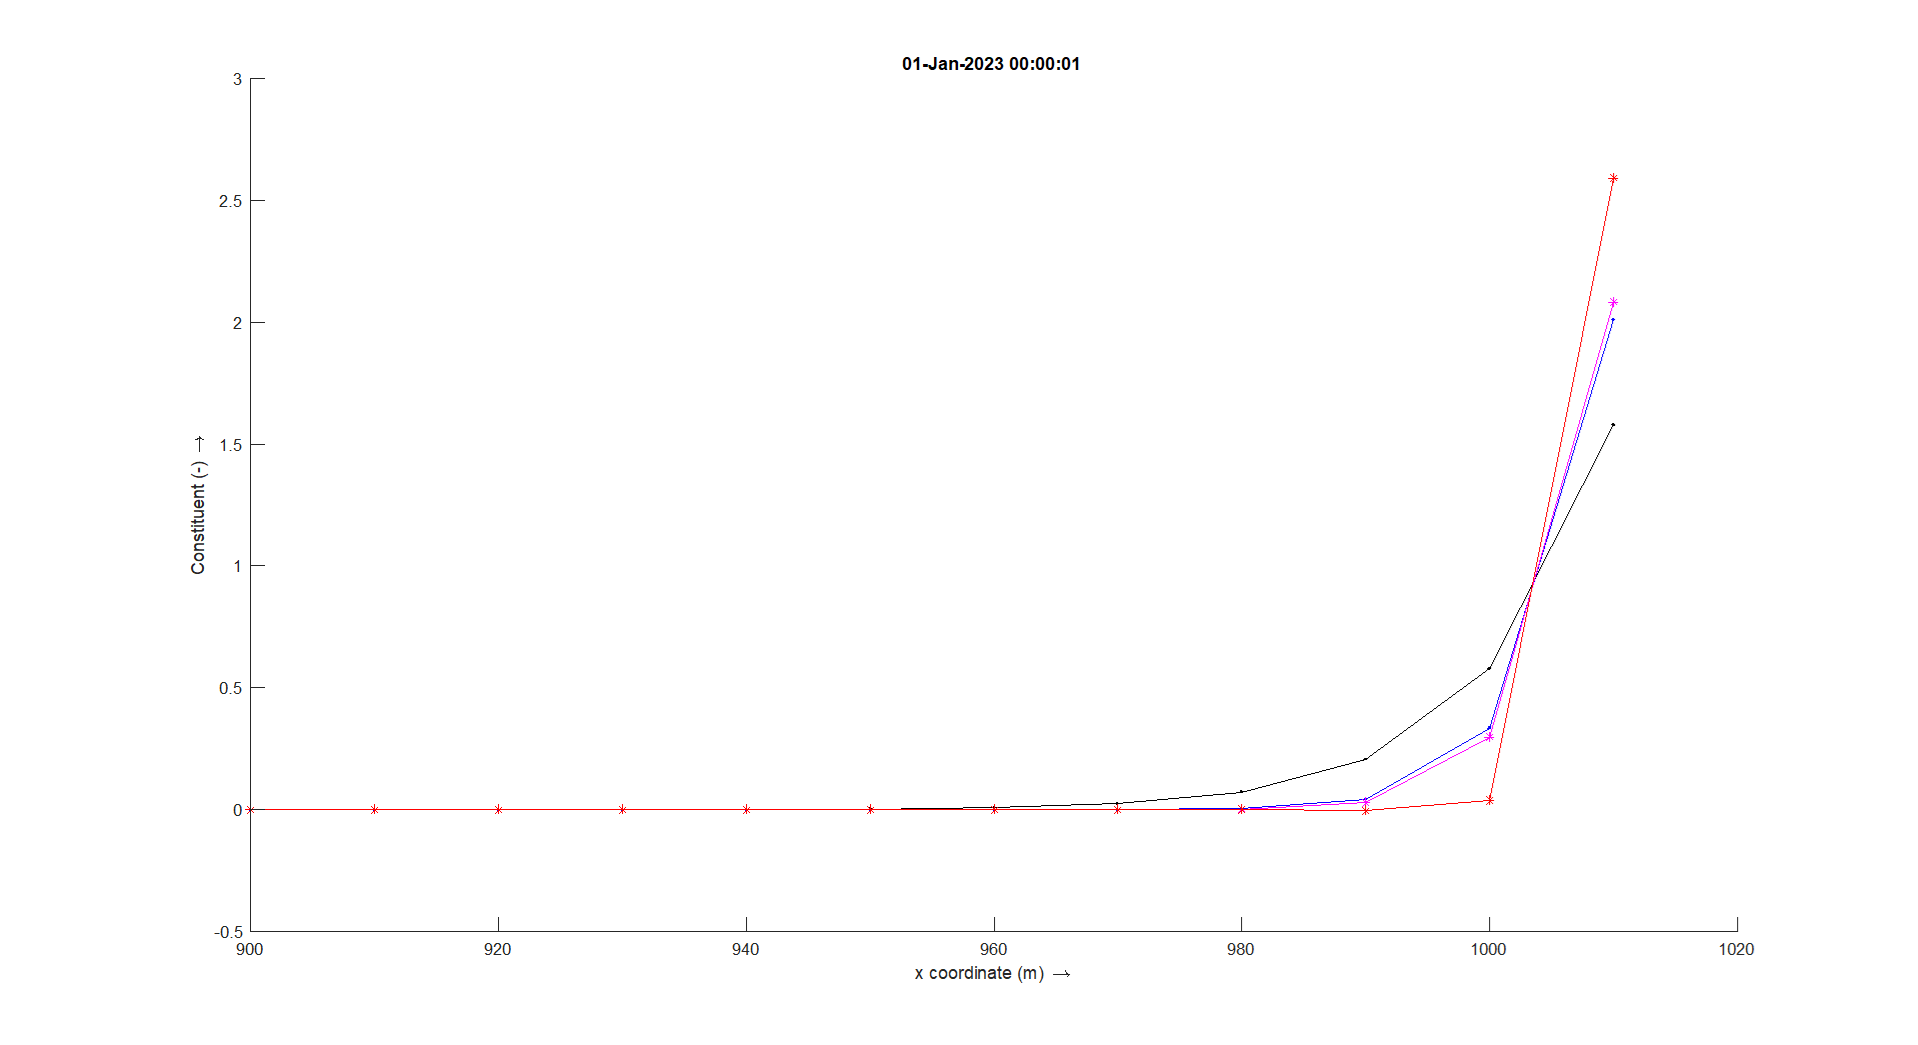
\includegraphics[width=0.9\textwidth]{figures/adv_diff_constituent.png}
    \caption{Numerical solution}
    \end{subfigure}
    \caption{Map results for different values of the advection velocity (thus P\'eclet number). The graphs with an  asterix represent results with a cell P\'eclet number larger then two. Black: $\Pe = 1.0$; Blue: $\Pe = 1.9$, Green: $\Pe = 2.1$; Cyan: $\Pe = 5.0$.}
\end{figure}
\begin{figure}[H]
    \centering
    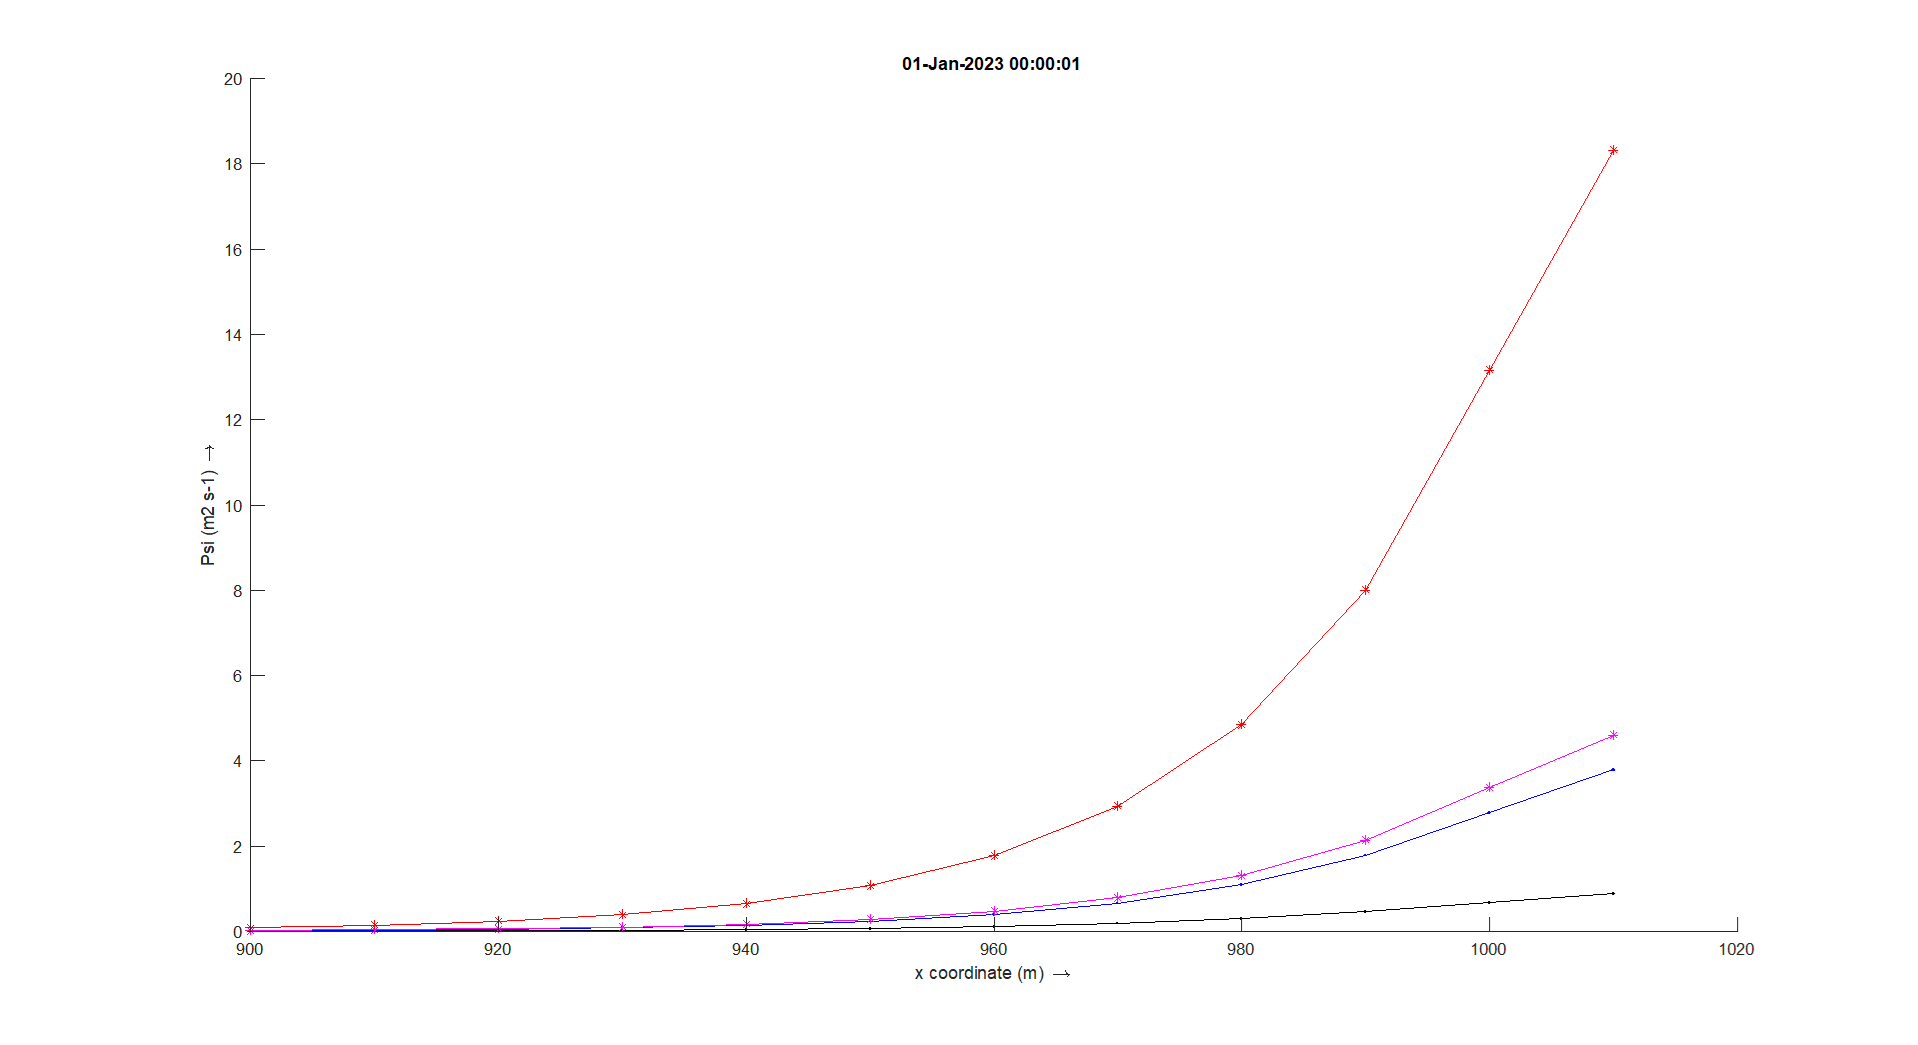
\includegraphics[width=0.9\textwidth]{figures/adv_diff_psi.png}
\caption{Map results for the used artificial diffusion $\Psi$. Black: $\Pe = 1.0$; Blue: $\Pe = 1.9$, Green: $\Pe = 2.1$; Cyan: $\Pe = 5.0$.}
\end{figure}
\begin{figure}[H]
    \centering
    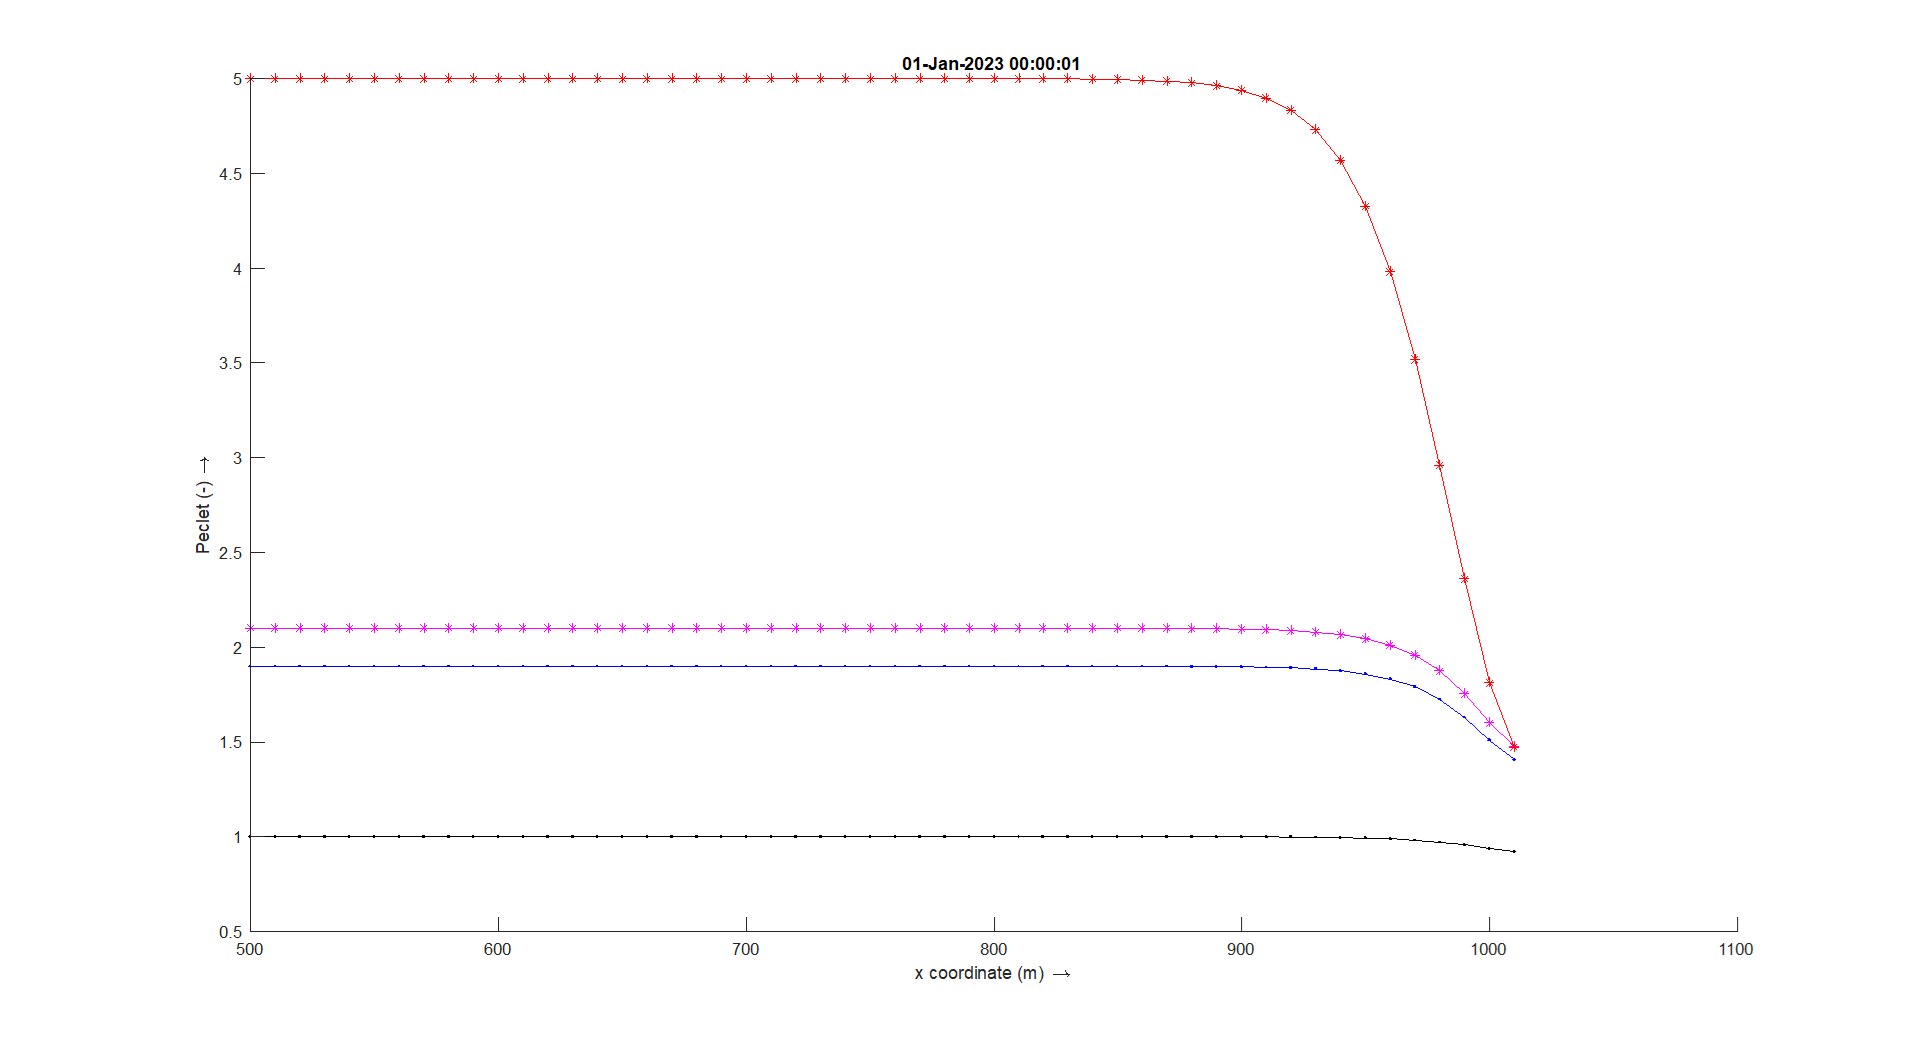
\includegraphics[width=0.9\textwidth]{figures/adv_diff_peclet.png}
    \caption{Map results for the used cell P\'eclet number. Black: $\Pe = 1.0$; Blue: $\Pe = 1.9$, Green: $\Pe = 2.1$; Cyan: $\Pe = 5.0$.}
\end{figure}

%--------------------------------------------------------------------------------
\subsection{Interface problem}\label{sec:1d_numerical_interface_experiment}
A numerical experiments is performed for the stationary advection-diffusion equation with a jump in the diffusion coefficient as described by:
\begin{align}
    \eps(x) &=
    \begin{cases}
        \check{\eps}, & \quad \text{if} \quad 0 < x \leq x^*, \\
        1, & \quad \text{if} \quad x^* < x < 1
    \end{cases}
\end{align}
An analytical solution exists in case $u=0$ and read \citep[eq.\ 3.11]{Wesseling2001}:
\begin{align}
    c(x)& =
    \begin{cases}
        \alpha x, & \quad \text{if} \quad 0 < x \leq x^*, \\
        \check{\eps}\alpha x + 1 - \check{\eps}\alpha, & \quad \text{if} \quad x^*<x<1
    \end{cases} \\
    \alpha & = \frac{1}{x^* -\check{\eps} x^* + \check{\eps}}
\end{align}

\begin{itemize}
    \item If $\eps \pdiff{c}{x} \equiv 0$ then either $\eps=0$ or $\pdiff{c}{x}=0$. Where $\eps=0$ is not feasible.
\end{itemize}

Some numerical experiments are performed with several values of $u$.

%--------------------------------------------------------------------------------
\paragraph*{Numerical experiment}
The numerical experiment is performed with the following parameters:
\begin{itemize}
    \item Length of the domain $L_x = \bqty{1}{\metre}$.
    \item Stationary simulation, $\lpdiff{c}{t}=0$.
    \item Prescribed boundary conditions: $c(0,t) = 0$ and $c(L_x,t) = 1$.
    \item Grid size: %  , $u = \bqty{0.9}{\metre\per\second}$
    \begin{itemize}
        \item $\Dx = \bqty{0.001}{\metre} \rightarrow \Pe = 0.09$,
        \item $\Dx = \bqty{0.01}{\metre} \rightarrow \Pe = 0.9$,
        \item $\Dx = \bqty{0.05}{\metre} \rightarrow \Pe = 4.5$,
    \end{itemize}
    \item Diffusion coefficient $\check{\eps} = \bqty{0.01}{\square\metre\per\second}$
    \item Advection velocities, $\Pe = u\Dx/\eps$:
    \begin{itemize}
        \item $u = \bqty{0}{\metre\per\second} \rightarrow \Pe = 0.0$
        \item $u = \bqty{0.9}{\metre\per\second} \rightarrow \Pe = 0.09, \Pe = 0.9\text{ and } \Pe = 4.5$
    \end{itemize}
\end{itemize}
%--------------------------------------------------------------------------------
\paragraph*{Results of numerical experiment}
Map results are presented for the constituent $c$ and the artificial diffusion $\Psi$.
\begin{figure}[H]
    \begin{subfigure}[t]{0.5\textwidth}
        \centering
        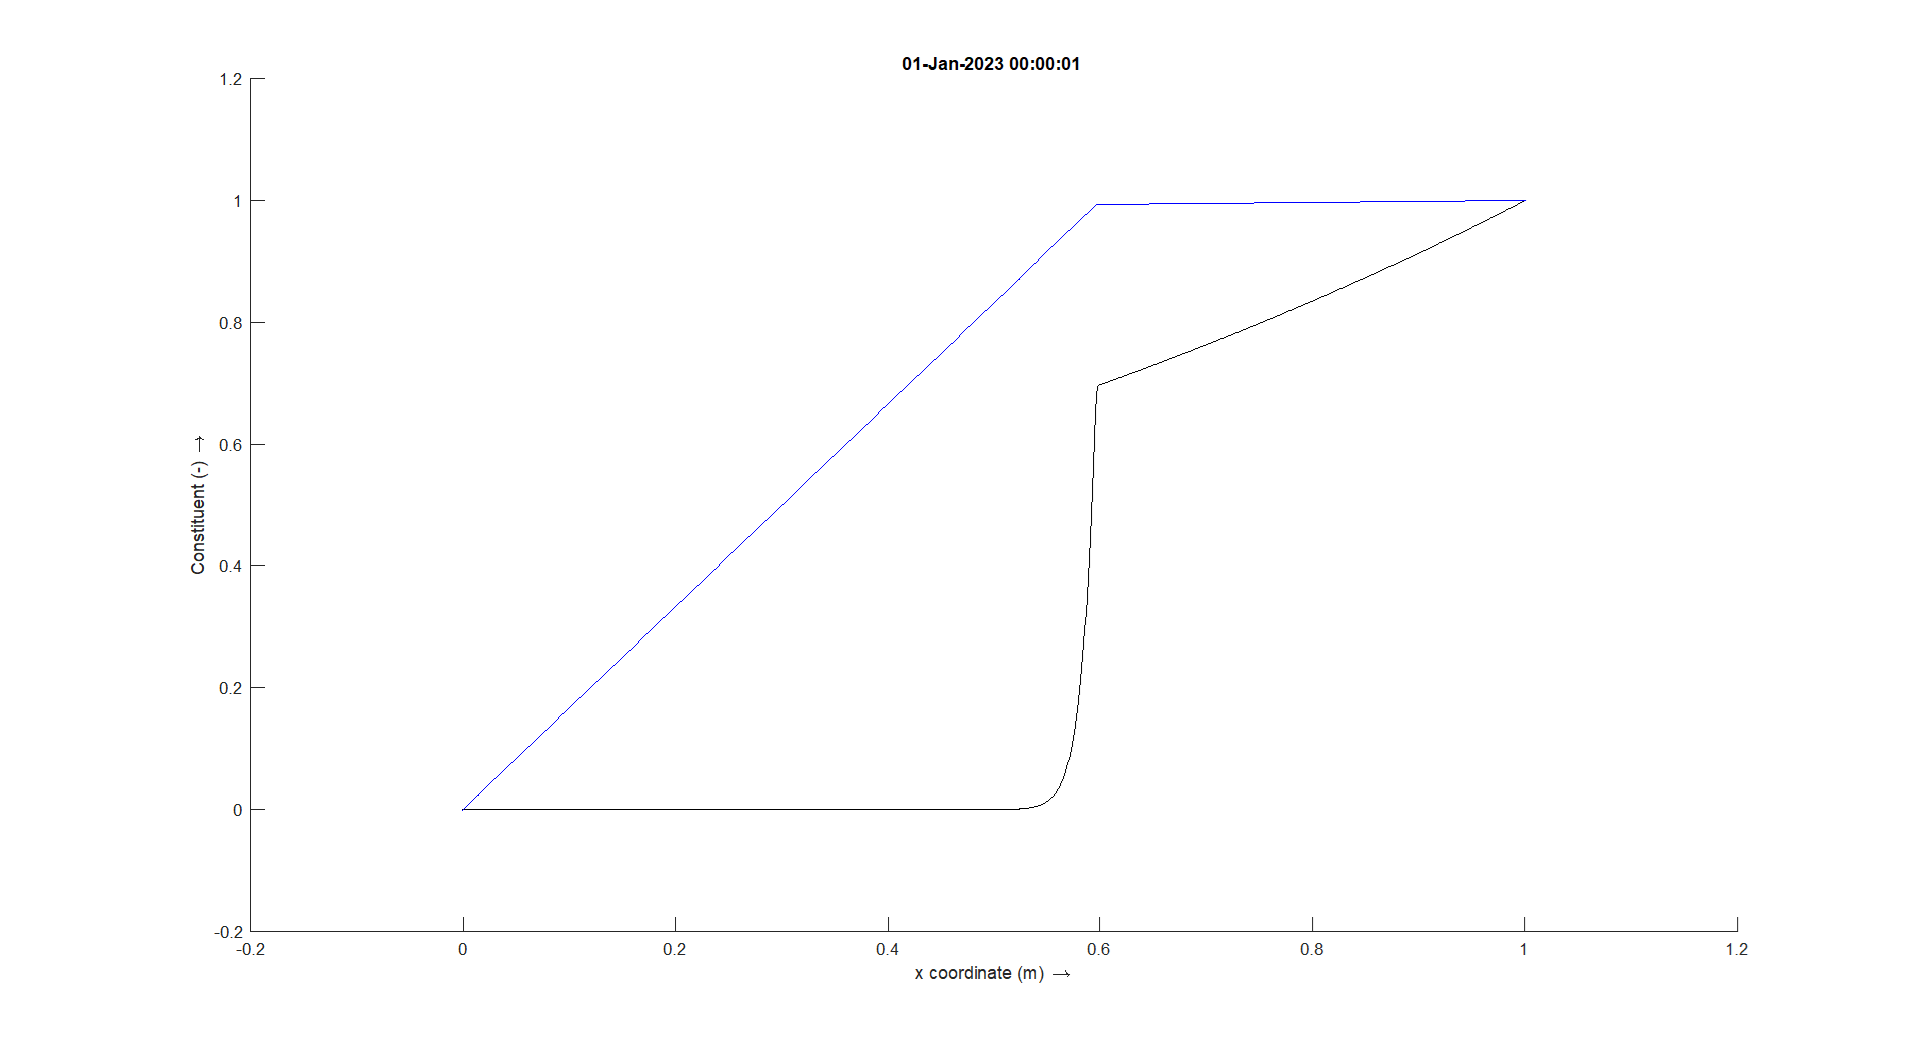
\includegraphics[width=0.9\textwidth]{figures/interface_u0d0_u0d9.png}
        \caption{High numerical resolution solution $\Dx=\bqty{0.001}{\metre}$.  Blue: $u =\bqty{0}{\metre\per\second}$ and Black: $u = \bqty{0.9}{\metre\per\second}$.}
    \end{subfigure}
    \hfill
    \begin{subfigure}[t]{0.5\textwidth}
        \centering
        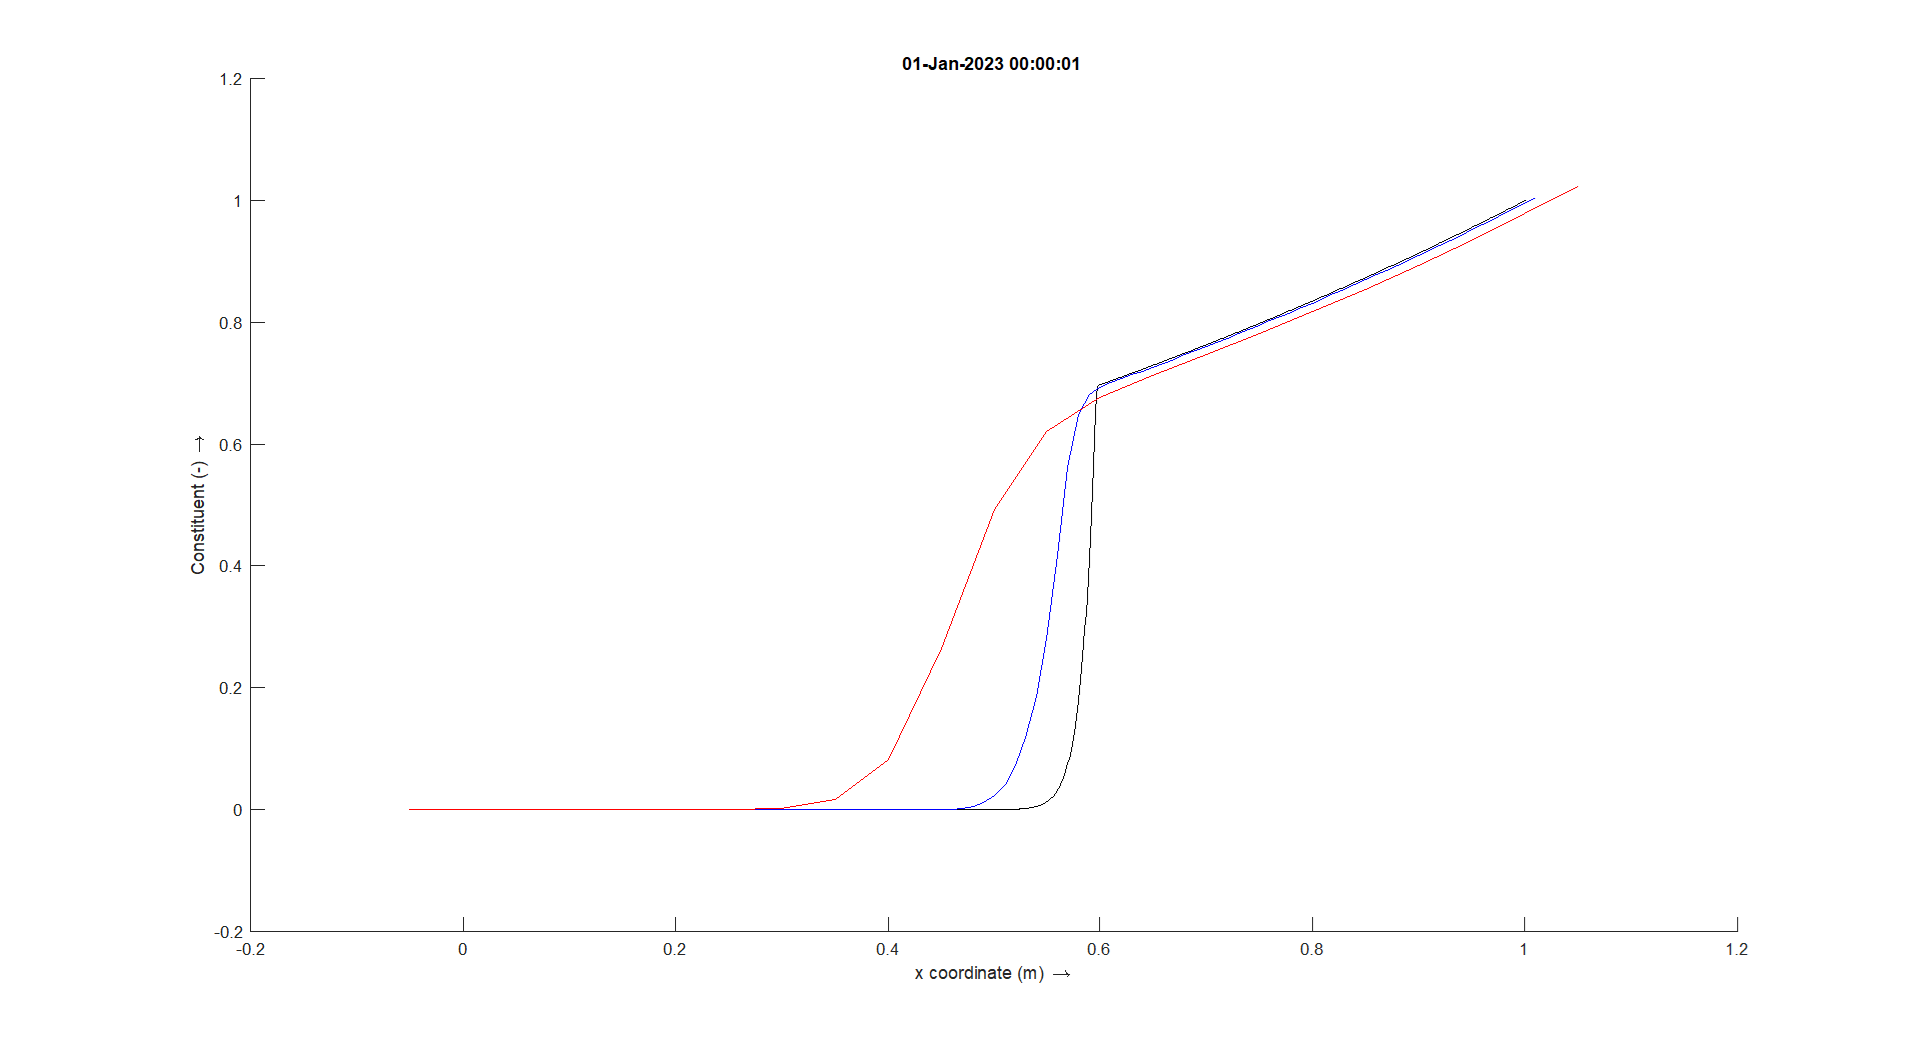
\includegraphics[width=0.9\textwidth]{figures/interface_pe0d09_pe0d9_pe4d5.png}
        \caption{Numerical solution, $u = \bqty{0.9}{\metre\per\second}$. Black: $\Dx = \bqty{0.001}{\metre} \rightarrow \Pe= 0.09$; Blue: $\Dx = \bqty{0.01}{\metre} \rightarrow \Pe = 0.9$ and Red: $\Dx = \bqty{0.05}{\metre} \rightarrow \Pe = 4.5$.}
    \end{subfigure}
    \caption{Map results for different values of the P\'eclet number.}
\end{figure}
%--------------------------------------------------------------------------------
\section{1-D Wave equation}
%--------------------------------------------------------------------------------
\subsection{Gaussian hump}\label{sec:numerical_experiment}
The considered 1-D wave equation reads:
\begin{align}
    \pdiff{h}{t}  + \pdiff{q}{x} & = 0 \qquad \textit{continuity eq.} \\
    \pdiff{q}{t}  + g h \pdiff{h}{x} & = 0 \qquad \textit{momentum eq.}
\end{align}
%
With initial conditions
\begin{align}
    h(x,0) & = \zeta(x,0) - z_b(x), \quad \bunit{\metre} \\
    q(x,0) & = 0, \quad \bunit{\square\metre\per\second}
\end{align}
for the the water level a Gaussian hump is prescribed
\begin{align}
    \zeta(x) = 2 a_0 \exp\left( \frac{(x - \mu)^2}{2\sigma^2}  \right), \quad \bunit{\metre}
\end{align}
At the boundaries no ingoing signals are prescribed, so outgoing signals are leaving the domain unhampered, which means no reflections will be present other then numerical reflections.
%--------------------------------------------------------------------------------
\paragraph*{Numerical experiment}
The numerical experiment is performed with the following parameters:
\begin{itemize}
    \item Length of the domain, $L_x = \bqty{12000}{\metre}$, ranging from $\bqty{-6000}{\metre}$ to $\bqty{6000}{\metre}$.
    \item Bed level, $z_b = \bqty{-10}{\metre}$.
    \item Grid size, $\Dx = \bqty{10}{\metre}$.
    \item Start time, $t_{start} = \bqty{0}{\second}$.
    \item End time, $t_{stop} = \bqty{3600}{\second}$.
    \item Timestep, $\Dt = \bqty{10}{\second}$.
    \item Regularization time for time-series, $t_{reg} = \bqty{300}{\second}$.
    \item Amplitude of the Gaussian hump at the boundary, $a_0 = \bqty{0.01}{\metre}$.
    \item Centre of the Gaussian hump, $\mu = \bqty{3000}{\metre}$.
    \item Spreading of the Gaussian hump, $\sigma = \bqty{700}{\metre}$.
\end{itemize}
And a second experiment with given boundary values:
\begin{itemize}
    \item Prescribed discharge boundary at $\bqty{-6000}{\metre}$: $q(0,t) = \bqty{0.05}{\square\metre\per\second}$.
    \item Prescribed water level boundary value at $\bqty{6000}{\metre}$: $\zeta(0,t) = \bqty{0.02}{\metre}$.
\end{itemize}
Because the boundary values are constant in time the solution is time-independent.
Therefore two simulation should be performed:
\begin{enumerate}
    \item A stationary computation (with $\Dt = \bqty{0}{\second}$) and
    \item an temporal computation (with $t_{stop} = \bqty{10800}{\second}$)
\end{enumerate}
%--------------------------------------------------------------------------------
\paragraph*{Results of the numerical experiments 1}
\notyet
%--------------------------------------------------------------------------------
\paragraph*{Results of the numerical experiments 2}
\notyet
%--------------------------------------------------------------------------------
\subsection{Weir}\label{sec:numerical_experiment_weir}
The model is taken from \citet{Borsboom2001}.
The considered 1-D wave equation reads:
\begin{align}
    \pdiff{h}{t} & + \pdiff{q}{x}  = 0, \qquad \textit{continuity eq.} \\
    \pdiff{q}{t} & + \pdiff{(q^2/h)}{x} + g h \pdiff{h}{x} - \pdiff{}{x} \left( (\nu+\Psi) h \pdiff{(q/h)}{x} \right) = 0, \qquad \textit{momentum eq.}
\end{align}
\begin{itemize}
    \item Length of the domain, $\bqty{500}{\metre}$.
    \item Artificial viscosity $\Psi$ computated as presented in \autoref{sec:regularization_artificial_viscosity}.
\end{itemize}
Bathymetry \bunit{\metre}:
\begin{align}
    z_b(x) =
    \begin{cases}
        \num{-12} & 0 < x \leq 200,
        \\
        \num{-12} + 7 (x - 200)/50 & 200 < x \leq 250,
        \\
        \num{-5} & 250 < x \leq 350,
        \\
        \num{-5} - 5(x - 350)/100 & 350 < x \leq 450,
        \\
        \num{-10} & 450 < x \leq 500.
    \end{cases}
\end{align}
Initial conditions
\begin{align}
    h(x,0) & = 0,\\
    q(x,0) & = 0
\end{align}
Boundary conditions
\begin{itemize}
    \item Prescribed discharge boundary at $\bqty{0}{\metre}$: $q(0,t) = \bqty{19.8656}{\square\metre\per\second}$.
    \item Prescribed water level boundary value at $\bqty{500}{\metre}$: $\zeta(500,t) = \bqty{-3}{\metre}$.
\end{itemize}
%--------------------------------------------------------------------------------
\paragraph*{Numerical experiment}
The numerical experiment is performed with the following parameters:
\begin{itemize}
    \item Grid size and time step,
    \begin{itemize}
        \item $\Dx = \bqty{10}{\metre}$ and $\Dt = \bqty{2}{s}$
        \item $\Dx = \bqty{5}{\metre}$ and $\Dt = \bqty{1}{s}$
        \item $\Dx = \bqty{2.5}{\metre}$ and $\Dt = \bqty{0.5}{s}$
        \item $\Dx = \bqty{1.25}{\metre}$ and $\Dt = \bqty{0.25}{s}$
    \end{itemize}
    \item Start time, $t_{start} = \bqty{0}{\second}$.
    \item End time, $t_{stop} = \bqty{7200}{\second}$.
    \item Regularization time for time-series, $t_{reg} = \bqty{300}{\second}$.
    \item Kinematic viscosity, $\nu = \bqty{0.01}{\square\metre\per\second}$
    \item $\eps_{bc} = \num{1e-02}$
\end{itemize}
%--------------------------------------------------------------------------------
\paragraph*{Results of the numerical experiments}
Results for the four different computations are shown in \autoref{fig:result_wl_weir}
\begin{figure}[H]
    \centering
    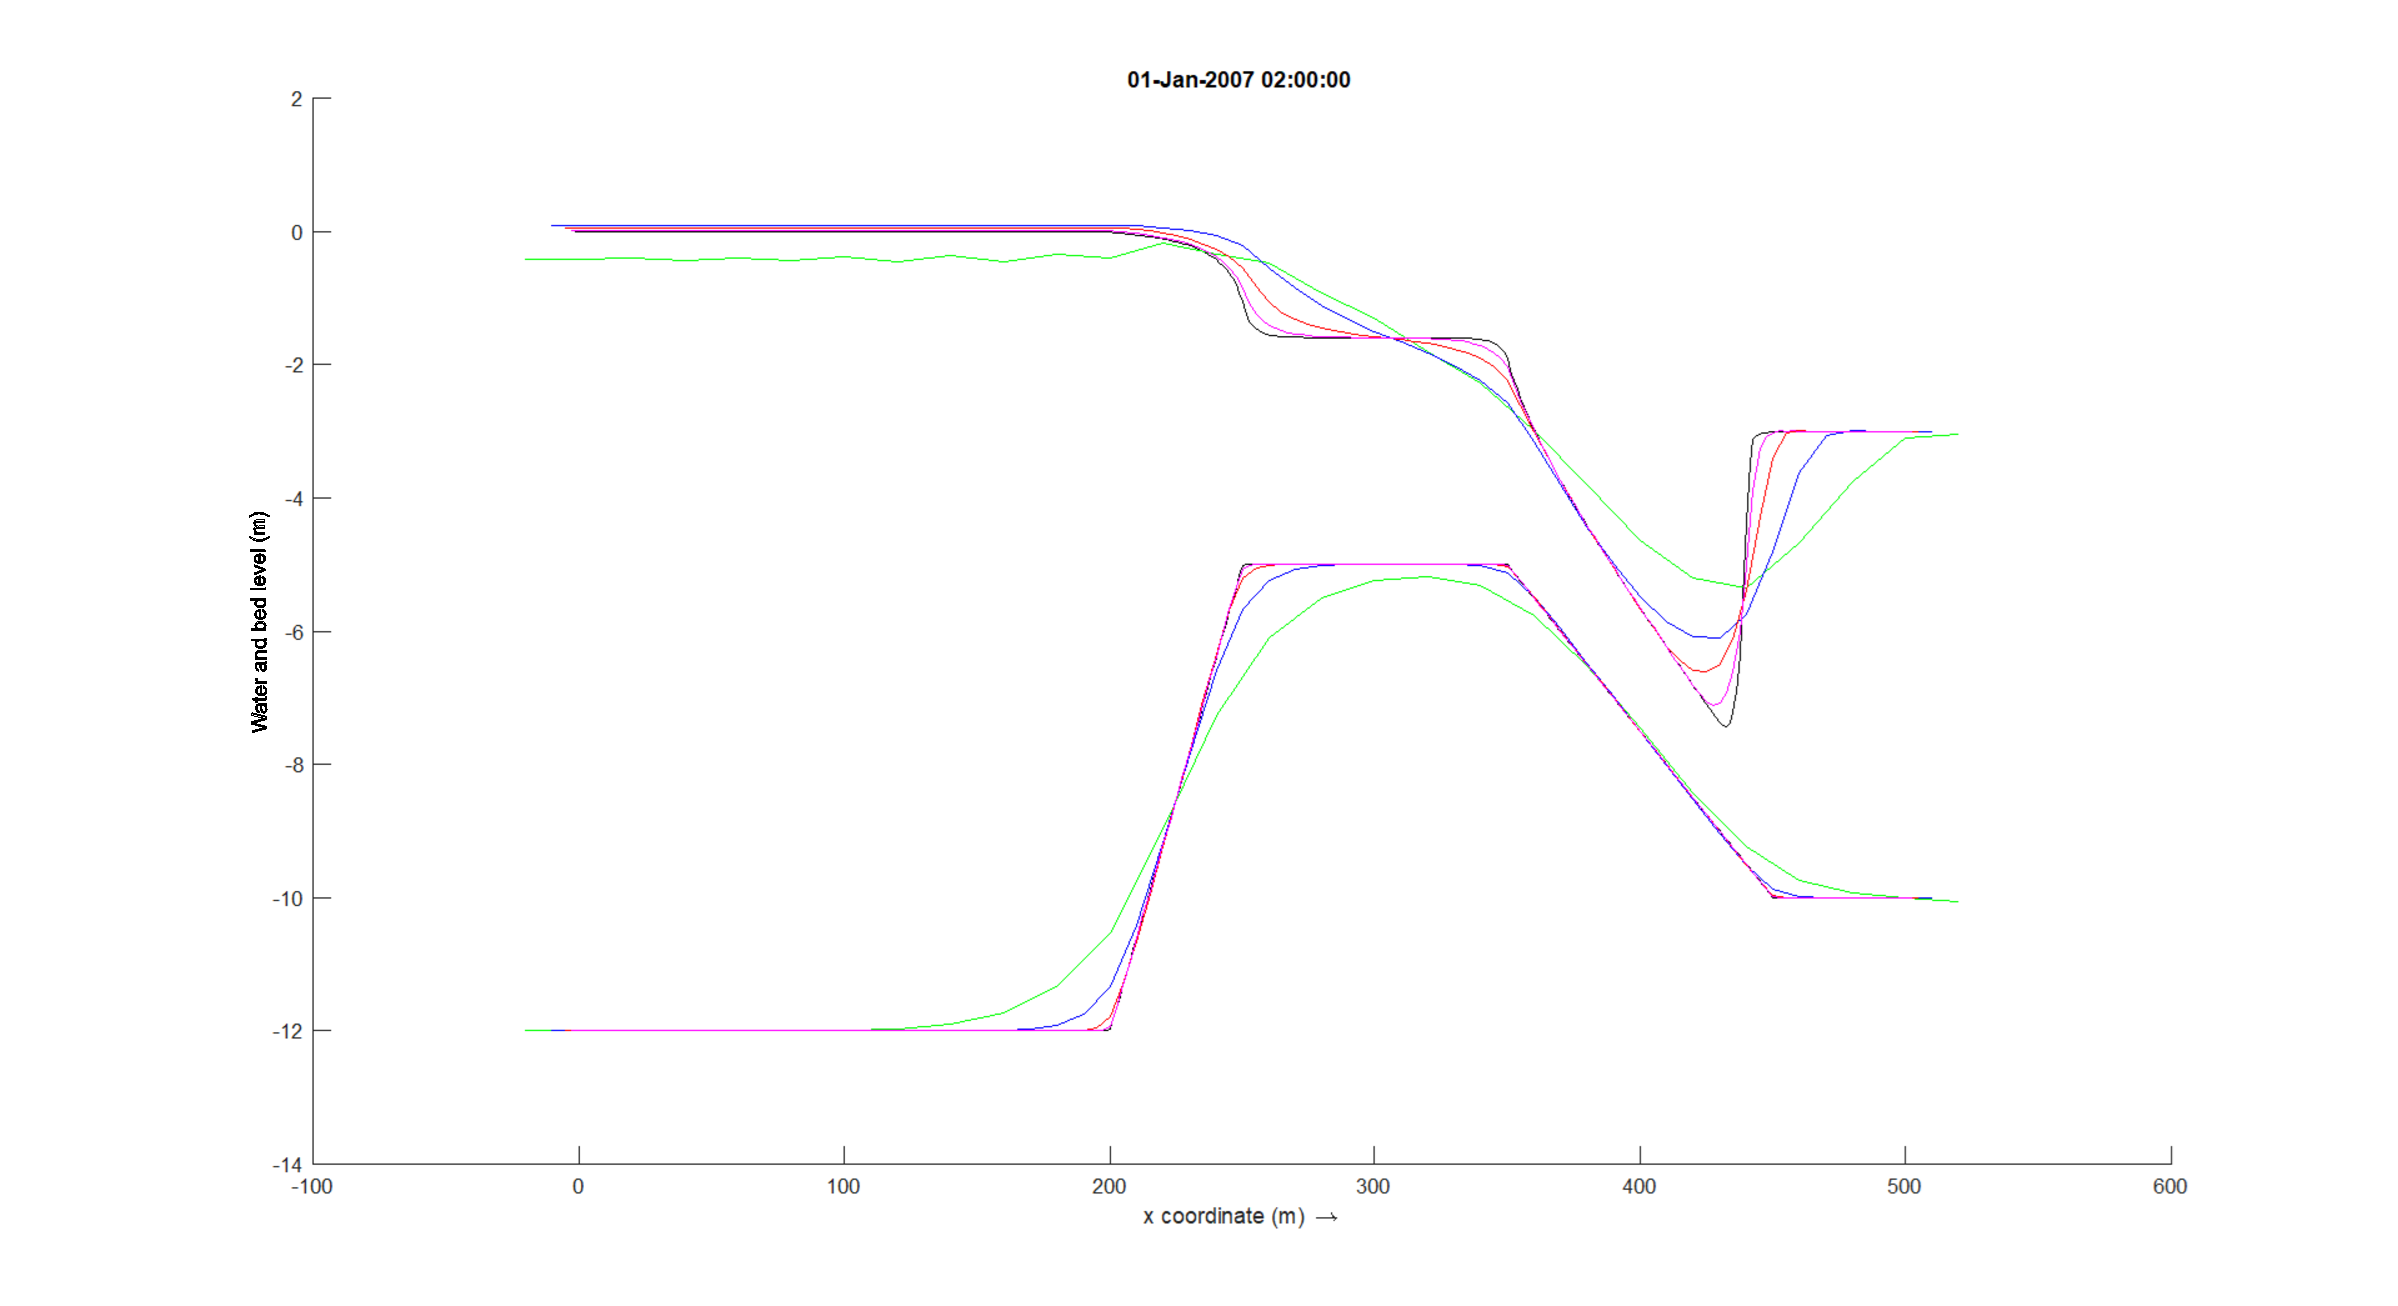
\includegraphics[width=0.9\textwidth]{figures/weir_bed_water_level.pdf}
    \caption[Weir experiment: water level and bed level]{Top graphs present the water level. Lower graphs present the regularized bathymetry.
    Green: $\Dx = \bqty{20}{\metre}$, $\Dt = \bqty{4}{\second}$;
    Blue: $\Dx = \bqty{10}{\metre}$, $\Dt = \bqty{2}{\second}$;
    Red: $\Dx = \bqty{5}{\metre}$, $\Dt = \bqty{1}{\second}$;
    Cyan: $\Dx = \bqty{2.5}{\metre}$, $\Dt = \bqty{0.5}{\second}$;
    Black: $\Dx = \bqty{1.25}{\metre}$, $\Dt =\bqty{0.25}{\second}$
    }
    \label{fig:result_wl_weir}
\end{figure}
%
\begin{figure}[H]
    \begin{subfigure}{0.5\textwidth}
        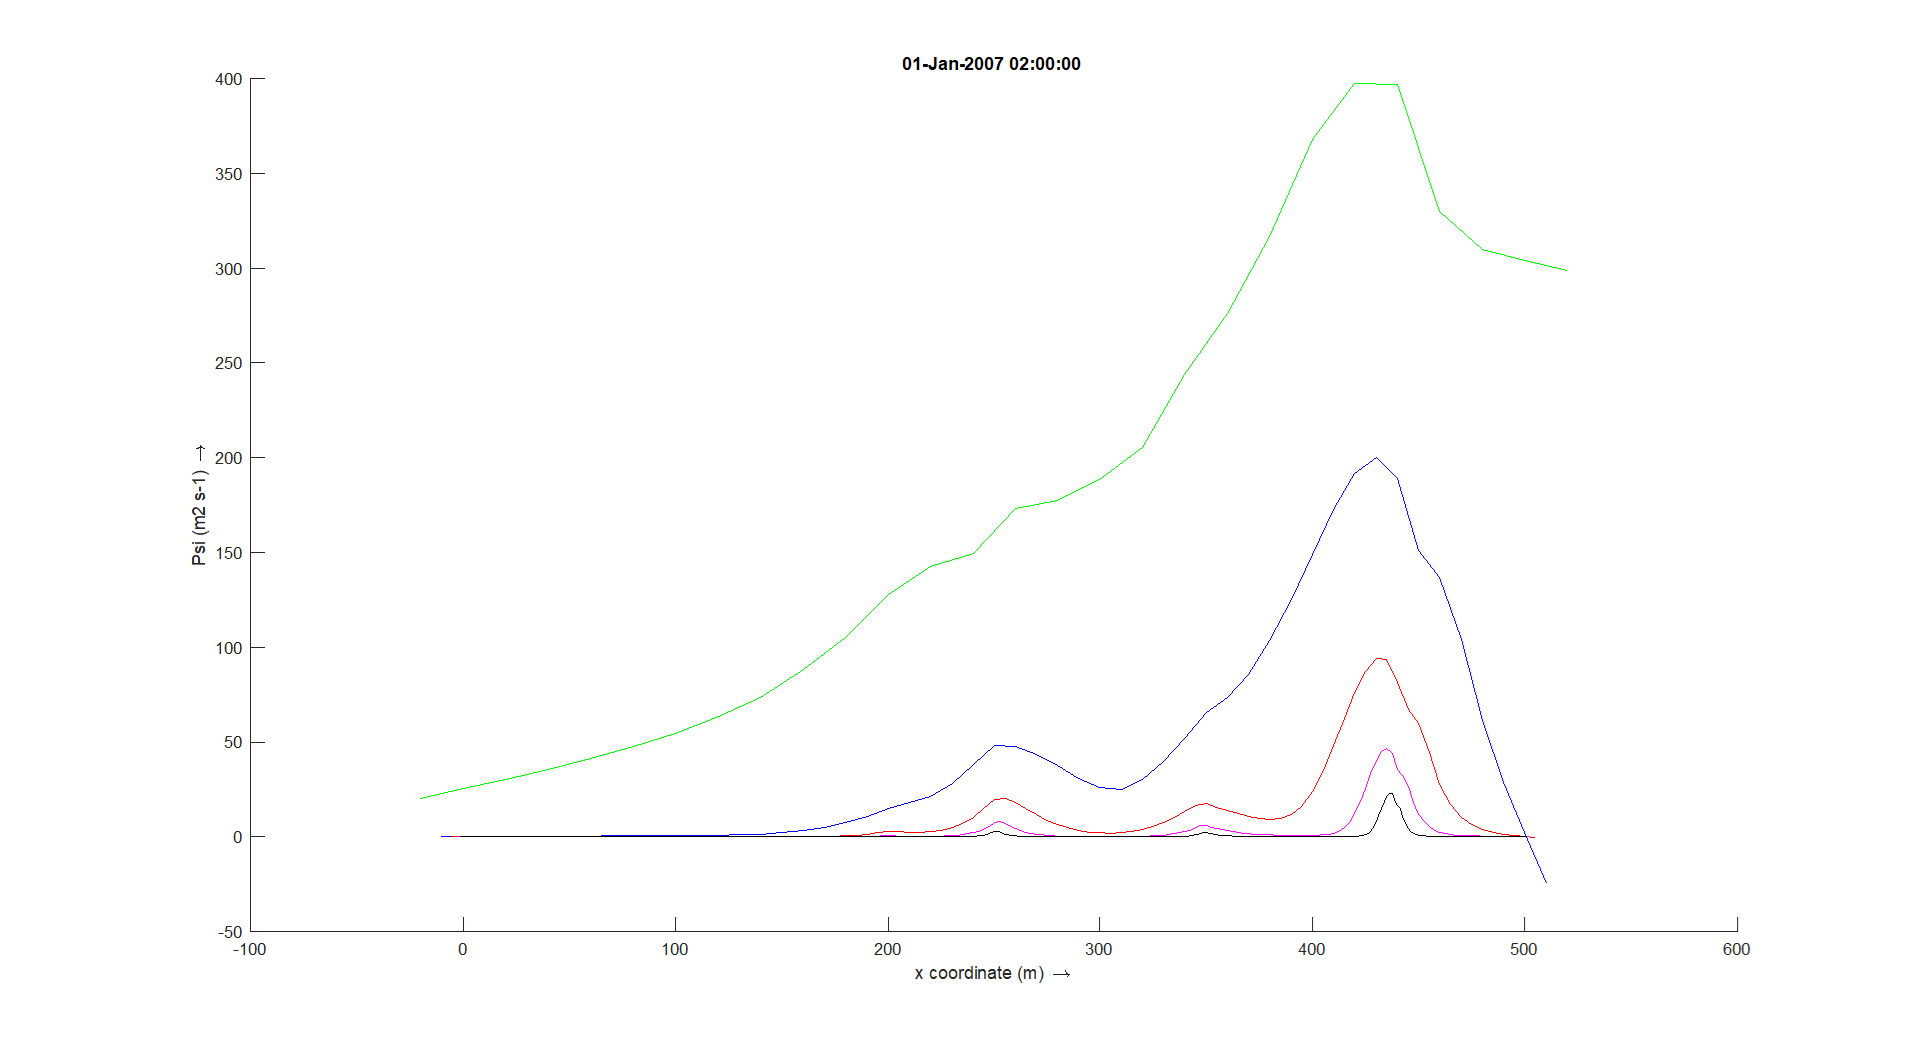
\includegraphics[width=\textwidth]{figures/weir_psi.png}
        \caption{Artificial viscosity $\Psi$.}
    \end{subfigure}
    \begin{subfigure}{0.5\textwidth}
        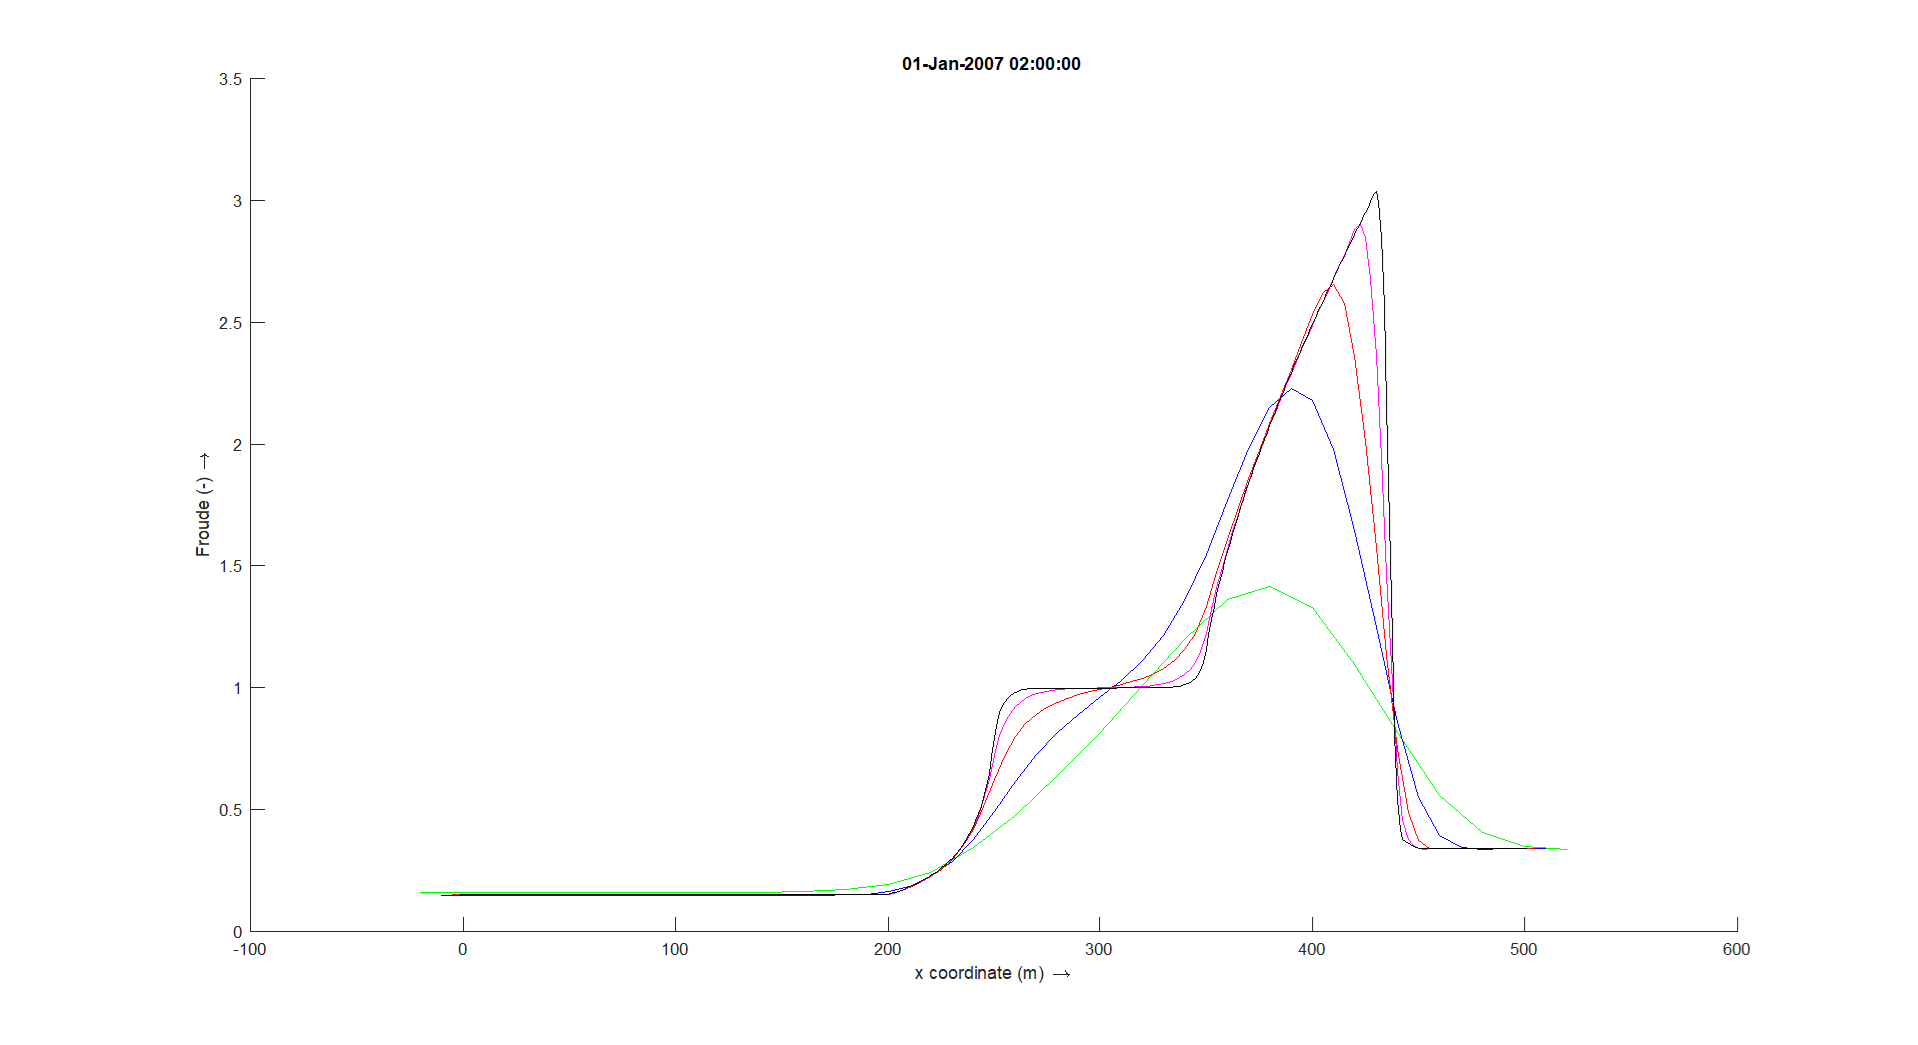
\includegraphics[width=\textwidth]{figures/weir_froude.png}
        \caption{Froude number.}
    \end{subfigure}
    \caption[Weir experiment: Artificial viscosity $\Psi$ and Froude number]{Artificial viscosity $\Psi$ and Froude number. Green: $\Dx = \bqty{20}{\metre}$, $\Dt = \bqty{4}{\second}$;
        Blue: $\Dx = \bqty{10}{\metre}$, $\Dt = \bqty{2}{\second}$;
        Red: $\Dx = \bqty{5}{\metre}$, $\Dt = \bqty{1}{\second}$;
        Cyan: $\Dx = \bqty{2.5}{\metre}$, $\Dt = \bqty{0.5}{\second}$;
        Black: $\Dx = \bqty{1.25}{\metre}$, $\Dt =\bqty{0.25}{\second}$
    }
\end{figure}
